\begin{figure}[H] \centering % Created by tikzDevice version 0.12.4 on 2023-08-13 18:11:34
% !TEX encoding = UTF-8 Unicode
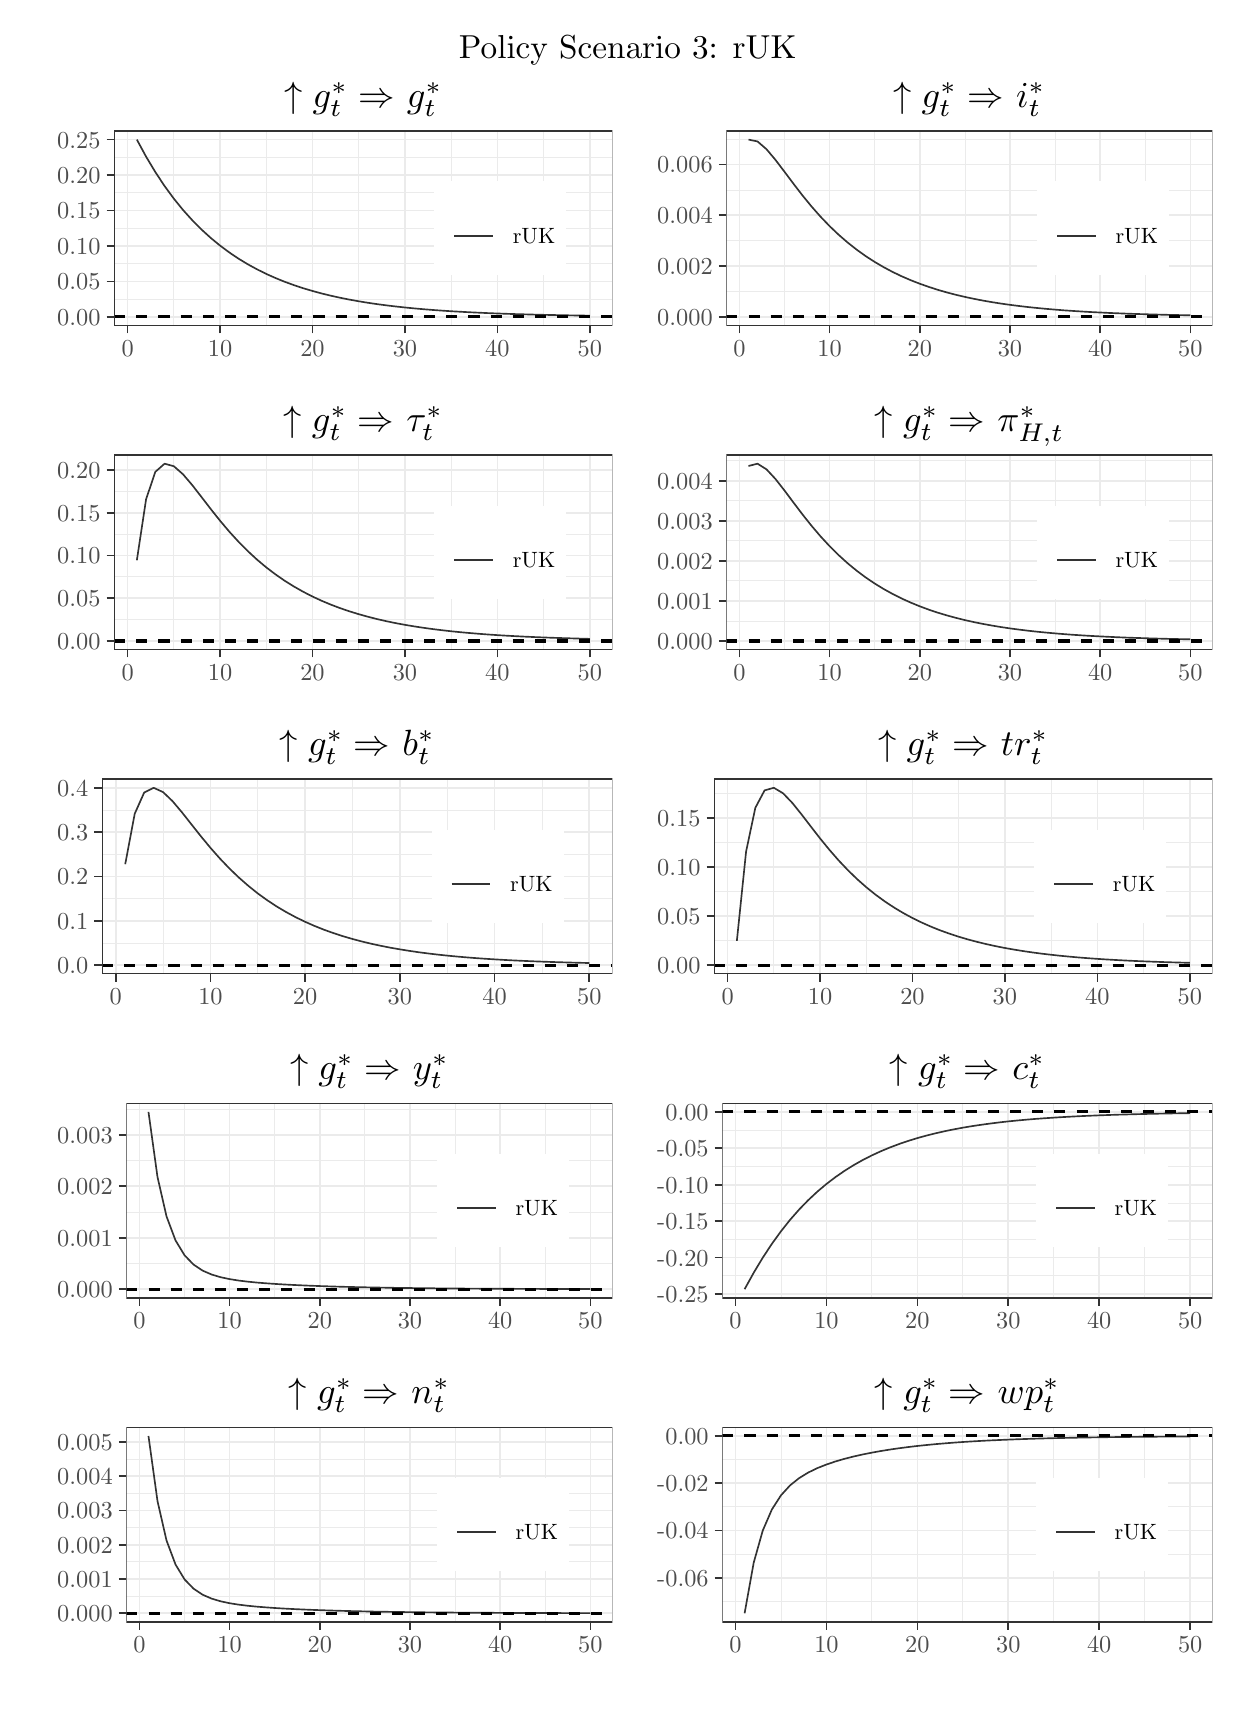
\begin{tikzpicture}[x=1pt,y=1pt]
\definecolor{fillColor}{RGB}{255,255,255}
\path[use as bounding box,fill=fillColor,fill opacity=0.00] (0,0) rectangle (433.62,599.84);
\begin{scope}
\path[clip] (  0.00,468.44) rectangle (216.81,585.55);
\definecolor{drawColor}{RGB}{255,255,255}
\definecolor{fillColor}{RGB}{255,255,255}

\path[draw=drawColor,line width= 0.6pt,line join=round,line cap=round,fill=fillColor] (  0.00,468.44) rectangle (216.81,585.55);
\end{scope}
\begin{scope}
\path[clip] ( 31.27,492.12) rectangle (211.31,562.59);
\definecolor{fillColor}{RGB}{255,255,255}

\path[fill=fillColor] ( 31.27,492.12) rectangle (211.31,562.59);
\definecolor{drawColor}{gray}{0.92}

\path[draw=drawColor,line width= 0.3pt,line join=round] ( 31.27,501.73) --
	(211.31,501.73);

\path[draw=drawColor,line width= 0.3pt,line join=round] ( 31.27,514.54) --
	(211.31,514.54);

\path[draw=drawColor,line width= 0.3pt,line join=round] ( 31.27,527.36) --
	(211.31,527.36);

\path[draw=drawColor,line width= 0.3pt,line join=round] ( 31.27,540.17) --
	(211.31,540.17);

\path[draw=drawColor,line width= 0.3pt,line join=round] ( 31.27,552.98) --
	(211.31,552.98);

\path[draw=drawColor,line width= 0.3pt,line join=round] ( 52.81,492.12) --
	( 52.81,562.59);

\path[draw=drawColor,line width= 0.3pt,line join=round] ( 86.22,492.12) --
	( 86.22,562.59);

\path[draw=drawColor,line width= 0.3pt,line join=round] (119.62,492.12) --
	(119.62,562.59);

\path[draw=drawColor,line width= 0.3pt,line join=round] (153.02,492.12) --
	(153.02,562.59);

\path[draw=drawColor,line width= 0.3pt,line join=round] (186.43,492.12) --
	(186.43,562.59);

\path[draw=drawColor,line width= 0.6pt,line join=round] ( 31.27,495.32) --
	(211.31,495.32);

\path[draw=drawColor,line width= 0.6pt,line join=round] ( 31.27,508.14) --
	(211.31,508.14);

\path[draw=drawColor,line width= 0.6pt,line join=round] ( 31.27,520.95) --
	(211.31,520.95);

\path[draw=drawColor,line width= 0.6pt,line join=round] ( 31.27,533.76) --
	(211.31,533.76);

\path[draw=drawColor,line width= 0.6pt,line join=round] ( 31.27,546.58) --
	(211.31,546.58);

\path[draw=drawColor,line width= 0.6pt,line join=round] ( 31.27,559.39) --
	(211.31,559.39);

\path[draw=drawColor,line width= 0.6pt,line join=round] ( 36.11,492.12) --
	( 36.11,562.59);

\path[draw=drawColor,line width= 0.6pt,line join=round] ( 69.52,492.12) --
	( 69.52,562.59);

\path[draw=drawColor,line width= 0.6pt,line join=round] (102.92,492.12) --
	(102.92,562.59);

\path[draw=drawColor,line width= 0.6pt,line join=round] (136.32,492.12) --
	(136.32,562.59);

\path[draw=drawColor,line width= 0.6pt,line join=round] (169.72,492.12) --
	(169.72,562.59);

\path[draw=drawColor,line width= 0.6pt,line join=round] (203.13,492.12) --
	(203.13,562.59);
\definecolor{drawColor}{gray}{0.20}

\path[draw=drawColor,line width= 0.6pt,line join=round] ( 39.45,559.39) --
	( 42.79,553.22) --
	( 46.13,547.65) --
	( 49.47,542.61) --
	( 52.81,538.06) --
	( 56.15,533.94) --
	( 59.50,530.23) --
	( 62.84,526.87) --
	( 66.18,523.83) --
	( 69.52,521.09) --
	( 72.86,518.61) --
	( 76.20,516.36) --
	( 79.54,514.34) --
	( 82.88,512.51) --
	( 86.22,510.85) --
	( 89.56,509.36) --
	( 92.90,508.01) --
	( 96.24,506.79) --
	( 99.58,505.68) --
	(102.92,504.69) --
	(106.26,503.78) --
	(109.60,502.97) --
	(112.94,502.23) --
	(116.28,501.57) --
	(119.62,500.97) --
	(122.96,500.42) --
	(126.30,499.93) --
	(129.64,499.49) --
	(132.98,499.09) --
	(136.32,498.73) --
	(139.66,498.40) --
	(143.00,498.10) --
	(146.34,497.83) --
	(149.68,497.59) --
	(153.02,497.37) --
	(156.36,497.18) --
	(159.70,497.00) --
	(163.04,496.84) --
	(166.38,496.69) --
	(169.72,496.56) --
	(173.06,496.44) --
	(176.40,496.33) --
	(179.74,496.24) --
	(183.08,496.15) --
	(186.43,496.07) --
	(189.77,496.00) --
	(193.11,495.93) --
	(196.45,495.87) --
	(199.79,495.82) --
	(203.13,495.77);
\definecolor{drawColor}{RGB}{0,0,0}

\path[draw=drawColor,line width= 1.1pt,dash pattern=on 4pt off 4pt ,line join=round] ( 31.27,495.32) -- (211.31,495.32);
\definecolor{drawColor}{gray}{0.20}

\path[draw=drawColor,line width= 0.6pt,line join=round,line cap=round] ( 31.27,492.12) rectangle (211.31,562.59);
\end{scope}
\begin{scope}
\path[clip] (  0.00,  0.00) rectangle (433.62,599.84);
\definecolor{drawColor}{gray}{0.30}

\node[text=drawColor,anchor=base east,inner sep=0pt, outer sep=0pt, scale=  0.88] at ( 26.32,492.29) {0.00};

\node[text=drawColor,anchor=base east,inner sep=0pt, outer sep=0pt, scale=  0.88] at ( 26.32,505.11) {0.05};

\node[text=drawColor,anchor=base east,inner sep=0pt, outer sep=0pt, scale=  0.88] at ( 26.32,517.92) {0.10};

\node[text=drawColor,anchor=base east,inner sep=0pt, outer sep=0pt, scale=  0.88] at ( 26.32,530.73) {0.15};

\node[text=drawColor,anchor=base east,inner sep=0pt, outer sep=0pt, scale=  0.88] at ( 26.32,543.55) {0.20};

\node[text=drawColor,anchor=base east,inner sep=0pt, outer sep=0pt, scale=  0.88] at ( 26.32,556.36) {0.25};
\end{scope}
\begin{scope}
\path[clip] (  0.00,  0.00) rectangle (433.62,599.84);
\definecolor{drawColor}{gray}{0.20}

\path[draw=drawColor,line width= 0.6pt,line join=round] ( 28.52,495.32) --
	( 31.27,495.32);

\path[draw=drawColor,line width= 0.6pt,line join=round] ( 28.52,508.14) --
	( 31.27,508.14);

\path[draw=drawColor,line width= 0.6pt,line join=round] ( 28.52,520.95) --
	( 31.27,520.95);

\path[draw=drawColor,line width= 0.6pt,line join=round] ( 28.52,533.76) --
	( 31.27,533.76);

\path[draw=drawColor,line width= 0.6pt,line join=round] ( 28.52,546.58) --
	( 31.27,546.58);

\path[draw=drawColor,line width= 0.6pt,line join=round] ( 28.52,559.39) --
	( 31.27,559.39);
\end{scope}
\begin{scope}
\path[clip] (  0.00,  0.00) rectangle (433.62,599.84);
\definecolor{drawColor}{gray}{0.20}

\path[draw=drawColor,line width= 0.6pt,line join=round] ( 36.11,489.37) --
	( 36.11,492.12);

\path[draw=drawColor,line width= 0.6pt,line join=round] ( 69.52,489.37) --
	( 69.52,492.12);

\path[draw=drawColor,line width= 0.6pt,line join=round] (102.92,489.37) --
	(102.92,492.12);

\path[draw=drawColor,line width= 0.6pt,line join=round] (136.32,489.37) --
	(136.32,492.12);

\path[draw=drawColor,line width= 0.6pt,line join=round] (169.72,489.37) --
	(169.72,492.12);

\path[draw=drawColor,line width= 0.6pt,line join=round] (203.13,489.37) --
	(203.13,492.12);
\end{scope}
\begin{scope}
\path[clip] (  0.00,  0.00) rectangle (433.62,599.84);
\definecolor{drawColor}{gray}{0.30}

\node[text=drawColor,anchor=base,inner sep=0pt, outer sep=0pt, scale=  0.88] at ( 36.11,481.11) {0};

\node[text=drawColor,anchor=base,inner sep=0pt, outer sep=0pt, scale=  0.88] at ( 69.52,481.11) {10};

\node[text=drawColor,anchor=base,inner sep=0pt, outer sep=0pt, scale=  0.88] at (102.92,481.11) {20};

\node[text=drawColor,anchor=base,inner sep=0pt, outer sep=0pt, scale=  0.88] at (136.32,481.11) {30};

\node[text=drawColor,anchor=base,inner sep=0pt, outer sep=0pt, scale=  0.88] at (169.72,481.11) {40};

\node[text=drawColor,anchor=base,inner sep=0pt, outer sep=0pt, scale=  0.88] at (203.13,481.11) {50};
\end{scope}
\begin{scope}
\path[clip] (  0.00,  0.00) rectangle (433.62,599.84);
\definecolor{fillColor}{RGB}{255,255,255}

\path[fill=fillColor] (146.96,510.43) rectangle (194.64,544.28);
\end{scope}
\begin{scope}
\path[clip] (  0.00,  0.00) rectangle (433.62,599.84);
\definecolor{fillColor}{RGB}{255,255,255}

\path[fill=fillColor] (152.46,515.93) rectangle (169.81,533.28);
\end{scope}
\begin{scope}
\path[clip] (  0.00,  0.00) rectangle (433.62,599.84);
\definecolor{drawColor}{gray}{0.20}

\path[draw=drawColor,line width= 0.6pt,line join=round] (154.20,524.61) -- (168.08,524.61);
\end{scope}
\begin{scope}
\path[clip] (  0.00,  0.00) rectangle (433.62,599.84);
\definecolor{drawColor}{RGB}{0,0,0}

\node[text=drawColor,anchor=base west,inner sep=0pt, outer sep=0pt, scale=  0.80] at (175.31,521.85) {rUK};
\end{scope}
\begin{scope}
\path[clip] (  0.00,  0.00) rectangle (433.62,599.84);
\definecolor{drawColor}{RGB}{0,0,0}

\node[text=drawColor,anchor=base,inner sep=0pt, outer sep=0pt, scale=  1.32] at (121.29,570.96) {$\uparrow  g^*_t \Rightarrow $ ${g^*_t}$};
\end{scope}
\begin{scope}
\path[clip] (216.81,468.44) rectangle (433.62,585.55);
\definecolor{drawColor}{RGB}{255,255,255}
\definecolor{fillColor}{RGB}{255,255,255}

\path[draw=drawColor,line width= 0.6pt,line join=round,line cap=round,fill=fillColor] (216.81,468.44) rectangle (433.62,585.55);
\end{scope}
\begin{scope}
\path[clip] (252.48,492.12) rectangle (428.12,562.59);
\definecolor{fillColor}{RGB}{255,255,255}

\path[fill=fillColor] (252.48,492.12) rectangle (428.12,562.59);
\definecolor{drawColor}{gray}{0.92}

\path[draw=drawColor,line width= 0.3pt,line join=round] (252.48,504.50) --
	(428.12,504.50);

\path[draw=drawColor,line width= 0.3pt,line join=round] (252.48,522.85) --
	(428.12,522.85);

\path[draw=drawColor,line width= 0.3pt,line join=round] (252.48,541.20) --
	(428.12,541.20);

\path[draw=drawColor,line width= 0.3pt,line join=round] (252.48,559.55) --
	(428.12,559.55);

\path[draw=drawColor,line width= 0.3pt,line join=round] (273.50,492.12) --
	(273.50,562.59);

\path[draw=drawColor,line width= 0.3pt,line join=round] (306.08,492.12) --
	(306.08,562.59);

\path[draw=drawColor,line width= 0.3pt,line join=round] (338.67,492.12) --
	(338.67,562.59);

\path[draw=drawColor,line width= 0.3pt,line join=round] (371.26,492.12) --
	(371.26,562.59);

\path[draw=drawColor,line width= 0.3pt,line join=round] (403.84,492.12) --
	(403.84,562.59);

\path[draw=drawColor,line width= 0.6pt,line join=round] (252.48,495.32) --
	(428.12,495.32);

\path[draw=drawColor,line width= 0.6pt,line join=round] (252.48,513.67) --
	(428.12,513.67);

\path[draw=drawColor,line width= 0.6pt,line join=round] (252.48,532.03) --
	(428.12,532.03);

\path[draw=drawColor,line width= 0.6pt,line join=round] (252.48,550.38) --
	(428.12,550.38);

\path[draw=drawColor,line width= 0.6pt,line join=round] (257.20,492.12) --
	(257.20,562.59);

\path[draw=drawColor,line width= 0.6pt,line join=round] (289.79,492.12) --
	(289.79,562.59);

\path[draw=drawColor,line width= 0.6pt,line join=round] (322.38,492.12) --
	(322.38,562.59);

\path[draw=drawColor,line width= 0.6pt,line join=round] (354.96,492.12) --
	(354.96,562.59);

\path[draw=drawColor,line width= 0.6pt,line join=round] (387.55,492.12) --
	(387.55,562.59);

\path[draw=drawColor,line width= 0.6pt,line join=round] (420.14,492.12) --
	(420.14,562.59);
\definecolor{drawColor}{gray}{0.20}

\path[draw=drawColor,line width= 0.6pt,line join=round] (260.46,559.39) --
	(263.72,558.73) --
	(266.98,555.90) --
	(270.24,552.03) --
	(273.50,547.73) --
	(276.76,543.38) --
	(280.01,539.17) --
	(283.27,535.19) --
	(286.53,531.50) --
	(289.79,528.11) --
	(293.05,525.00) --
	(296.31,522.18) --
	(299.57,519.61) --
	(302.82,517.28) --
	(306.08,515.18) --
	(309.34,513.27) --
	(312.60,511.54) --
	(315.86,509.98) --
	(319.12,508.57) --
	(322.38,507.30) --
	(325.64,506.15) --
	(328.89,505.10) --
	(332.15,504.16) --
	(335.41,503.31) --
	(338.67,502.54) --
	(341.93,501.85) --
	(345.19,501.22) --
	(348.45,500.65) --
	(351.70,500.14) --
	(354.96,499.68) --
	(358.22,499.26) --
	(361.48,498.88) --
	(364.74,498.54) --
	(368.00,498.23) --
	(371.26,497.95) --
	(374.52,497.69) --
	(377.77,497.47) --
	(381.03,497.26) --
	(384.29,497.07) --
	(387.55,496.91) --
	(390.81,496.75) --
	(394.07,496.62) --
	(397.33,496.49) --
	(400.58,496.38) --
	(403.84,496.28) --
	(407.10,496.19) --
	(410.36,496.10) --
	(413.62,496.03) --
	(416.88,495.96) --
	(420.14,495.90);
\definecolor{drawColor}{RGB}{0,0,0}

\path[draw=drawColor,line width= 1.1pt,dash pattern=on 4pt off 4pt ,line join=round] (252.48,495.32) -- (428.12,495.32);
\definecolor{drawColor}{gray}{0.20}

\path[draw=drawColor,line width= 0.6pt,line join=round,line cap=round] (252.48,492.12) rectangle (428.12,562.59);
\end{scope}
\begin{scope}
\path[clip] (  0.00,  0.00) rectangle (433.62,599.84);
\definecolor{drawColor}{gray}{0.30}

\node[text=drawColor,anchor=base east,inner sep=0pt, outer sep=0pt, scale=  0.88] at (247.53,492.29) {0.000};

\node[text=drawColor,anchor=base east,inner sep=0pt, outer sep=0pt, scale=  0.88] at (247.53,510.64) {0.002};

\node[text=drawColor,anchor=base east,inner sep=0pt, outer sep=0pt, scale=  0.88] at (247.53,529.00) {0.004};

\node[text=drawColor,anchor=base east,inner sep=0pt, outer sep=0pt, scale=  0.88] at (247.53,547.35) {0.006};
\end{scope}
\begin{scope}
\path[clip] (  0.00,  0.00) rectangle (433.62,599.84);
\definecolor{drawColor}{gray}{0.20}

\path[draw=drawColor,line width= 0.6pt,line join=round] (249.73,495.32) --
	(252.48,495.32);

\path[draw=drawColor,line width= 0.6pt,line join=round] (249.73,513.67) --
	(252.48,513.67);

\path[draw=drawColor,line width= 0.6pt,line join=round] (249.73,532.03) --
	(252.48,532.03);

\path[draw=drawColor,line width= 0.6pt,line join=round] (249.73,550.38) --
	(252.48,550.38);
\end{scope}
\begin{scope}
\path[clip] (  0.00,  0.00) rectangle (433.62,599.84);
\definecolor{drawColor}{gray}{0.20}

\path[draw=drawColor,line width= 0.6pt,line join=round] (257.20,489.37) --
	(257.20,492.12);

\path[draw=drawColor,line width= 0.6pt,line join=round] (289.79,489.37) --
	(289.79,492.12);

\path[draw=drawColor,line width= 0.6pt,line join=round] (322.38,489.37) --
	(322.38,492.12);

\path[draw=drawColor,line width= 0.6pt,line join=round] (354.96,489.37) --
	(354.96,492.12);

\path[draw=drawColor,line width= 0.6pt,line join=round] (387.55,489.37) --
	(387.55,492.12);

\path[draw=drawColor,line width= 0.6pt,line join=round] (420.14,489.37) --
	(420.14,492.12);
\end{scope}
\begin{scope}
\path[clip] (  0.00,  0.00) rectangle (433.62,599.84);
\definecolor{drawColor}{gray}{0.30}

\node[text=drawColor,anchor=base,inner sep=0pt, outer sep=0pt, scale=  0.88] at (257.20,481.11) {0};

\node[text=drawColor,anchor=base,inner sep=0pt, outer sep=0pt, scale=  0.88] at (289.79,481.11) {10};

\node[text=drawColor,anchor=base,inner sep=0pt, outer sep=0pt, scale=  0.88] at (322.38,481.11) {20};

\node[text=drawColor,anchor=base,inner sep=0pt, outer sep=0pt, scale=  0.88] at (354.96,481.11) {30};

\node[text=drawColor,anchor=base,inner sep=0pt, outer sep=0pt, scale=  0.88] at (387.55,481.11) {40};

\node[text=drawColor,anchor=base,inner sep=0pt, outer sep=0pt, scale=  0.88] at (420.14,481.11) {50};
\end{scope}
\begin{scope}
\path[clip] (  0.00,  0.00) rectangle (433.62,599.84);
\definecolor{fillColor}{RGB}{255,255,255}

\path[fill=fillColor] (364.76,510.43) rectangle (412.44,544.28);
\end{scope}
\begin{scope}
\path[clip] (  0.00,  0.00) rectangle (433.62,599.84);
\definecolor{fillColor}{RGB}{255,255,255}

\path[fill=fillColor] (370.26,515.93) rectangle (387.61,533.28);
\end{scope}
\begin{scope}
\path[clip] (  0.00,  0.00) rectangle (433.62,599.84);
\definecolor{drawColor}{gray}{0.20}

\path[draw=drawColor,line width= 0.6pt,line join=round] (372.00,524.61) -- (385.87,524.61);
\end{scope}
\begin{scope}
\path[clip] (  0.00,  0.00) rectangle (433.62,599.84);
\definecolor{drawColor}{RGB}{0,0,0}

\node[text=drawColor,anchor=base west,inner sep=0pt, outer sep=0pt, scale=  0.80] at (393.11,521.85) {rUK};
\end{scope}
\begin{scope}
\path[clip] (  0.00,  0.00) rectangle (433.62,599.84);
\definecolor{drawColor}{RGB}{0,0,0}

\node[text=drawColor,anchor=base,inner sep=0pt, outer sep=0pt, scale=  1.32] at (340.30,570.96) {$\uparrow  g^*_t \Rightarrow $ ${i^*_t}$};
\end{scope}
\begin{scope}
\path[clip] (  0.00,351.33) rectangle (216.81,468.44);
\definecolor{drawColor}{RGB}{255,255,255}
\definecolor{fillColor}{RGB}{255,255,255}

\path[draw=drawColor,line width= 0.6pt,line join=round,line cap=round,fill=fillColor] (  0.00,351.33) rectangle (216.81,468.44);
\end{scope}
\begin{scope}
\path[clip] ( 31.27,375.01) rectangle (211.31,445.48);
\definecolor{fillColor}{RGB}{255,255,255}

\path[fill=fillColor] ( 31.27,375.01) rectangle (211.31,445.48);
\definecolor{drawColor}{gray}{0.92}

\path[draw=drawColor,line width= 0.3pt,line join=round] ( 31.27,385.93) --
	(211.31,385.93);

\path[draw=drawColor,line width= 0.3pt,line join=round] ( 31.27,401.37) --
	(211.31,401.37);

\path[draw=drawColor,line width= 0.3pt,line join=round] ( 31.27,416.81) --
	(211.31,416.81);

\path[draw=drawColor,line width= 0.3pt,line join=round] ( 31.27,432.24) --
	(211.31,432.24);

\path[draw=drawColor,line width= 0.3pt,line join=round] ( 52.81,375.01) --
	( 52.81,445.48);

\path[draw=drawColor,line width= 0.3pt,line join=round] ( 86.22,375.01) --
	( 86.22,445.48);

\path[draw=drawColor,line width= 0.3pt,line join=round] (119.62,375.01) --
	(119.62,445.48);

\path[draw=drawColor,line width= 0.3pt,line join=round] (153.02,375.01) --
	(153.02,445.48);

\path[draw=drawColor,line width= 0.3pt,line join=round] (186.43,375.01) --
	(186.43,445.48);

\path[draw=drawColor,line width= 0.6pt,line join=round] ( 31.27,378.21) --
	(211.31,378.21);

\path[draw=drawColor,line width= 0.6pt,line join=round] ( 31.27,393.65) --
	(211.31,393.65);

\path[draw=drawColor,line width= 0.6pt,line join=round] ( 31.27,409.09) --
	(211.31,409.09);

\path[draw=drawColor,line width= 0.6pt,line join=round] ( 31.27,424.52) --
	(211.31,424.52);

\path[draw=drawColor,line width= 0.6pt,line join=round] ( 31.27,439.96) --
	(211.31,439.96);

\path[draw=drawColor,line width= 0.6pt,line join=round] ( 36.11,375.01) --
	( 36.11,445.48);

\path[draw=drawColor,line width= 0.6pt,line join=round] ( 69.52,375.01) --
	( 69.52,445.48);

\path[draw=drawColor,line width= 0.6pt,line join=round] (102.92,375.01) --
	(102.92,445.48);

\path[draw=drawColor,line width= 0.6pt,line join=round] (136.32,375.01) --
	(136.32,445.48);

\path[draw=drawColor,line width= 0.6pt,line join=round] (169.72,375.01) --
	(169.72,445.48);

\path[draw=drawColor,line width= 0.6pt,line join=round] (203.13,375.01) --
	(203.13,445.48);
\definecolor{drawColor}{gray}{0.20}

\path[draw=drawColor,line width= 0.6pt,line join=round] ( 39.45,407.37) --
	( 42.79,429.44) --
	( 46.13,439.33) --
	( 49.47,442.28) --
	( 52.81,441.37) --
	( 56.15,438.43) --
	( 59.50,434.50) --
	( 62.84,430.20) --
	( 66.18,425.86) --
	( 69.52,421.67) --
	( 72.86,417.72) --
	( 76.20,414.06) --
	( 79.54,410.69) --
	( 82.88,407.61) --
	( 86.22,404.81) --
	( 89.56,402.27) --
	( 92.90,399.96) --
	( 96.24,397.88) --
	( 99.58,395.99) --
	(102.92,394.28) --
	(106.26,392.73) --
	(109.60,391.33) --
	(112.94,390.07) --
	(116.28,388.93) --
	(119.62,387.90) --
	(122.96,386.97) --
	(126.30,386.12) --
	(129.64,385.36) --
	(132.98,384.67) --
	(136.32,384.05) --
	(139.66,383.49) --
	(143.00,382.98) --
	(146.34,382.52) --
	(149.68,382.11) --
	(153.02,381.73) --
	(156.36,381.39) --
	(159.70,381.09) --
	(163.04,380.81) --
	(166.38,380.56) --
	(169.72,380.33) --
	(173.06,380.13) --
	(176.40,379.95) --
	(179.74,379.78) --
	(183.08,379.63) --
	(186.43,379.49) --
	(189.77,379.37) --
	(193.11,379.26) --
	(196.45,379.16) --
	(199.79,379.07) --
	(203.13,378.98);
\definecolor{drawColor}{RGB}{0,0,0}

\path[draw=drawColor,line width= 1.1pt,dash pattern=on 4pt off 4pt ,line join=round] ( 31.27,378.21) -- (211.31,378.21);
\definecolor{drawColor}{gray}{0.20}

\path[draw=drawColor,line width= 0.6pt,line join=round,line cap=round] ( 31.27,375.01) rectangle (211.31,445.48);
\end{scope}
\begin{scope}
\path[clip] (  0.00,  0.00) rectangle (433.62,599.84);
\definecolor{drawColor}{gray}{0.30}

\node[text=drawColor,anchor=base east,inner sep=0pt, outer sep=0pt, scale=  0.88] at ( 26.32,375.18) {0.00};

\node[text=drawColor,anchor=base east,inner sep=0pt, outer sep=0pt, scale=  0.88] at ( 26.32,390.62) {0.05};

\node[text=drawColor,anchor=base east,inner sep=0pt, outer sep=0pt, scale=  0.88] at ( 26.32,406.06) {0.10};

\node[text=drawColor,anchor=base east,inner sep=0pt, outer sep=0pt, scale=  0.88] at ( 26.32,421.49) {0.15};

\node[text=drawColor,anchor=base east,inner sep=0pt, outer sep=0pt, scale=  0.88] at ( 26.32,436.93) {0.20};
\end{scope}
\begin{scope}
\path[clip] (  0.00,  0.00) rectangle (433.62,599.84);
\definecolor{drawColor}{gray}{0.20}

\path[draw=drawColor,line width= 0.6pt,line join=round] ( 28.52,378.21) --
	( 31.27,378.21);

\path[draw=drawColor,line width= 0.6pt,line join=round] ( 28.52,393.65) --
	( 31.27,393.65);

\path[draw=drawColor,line width= 0.6pt,line join=round] ( 28.52,409.09) --
	( 31.27,409.09);

\path[draw=drawColor,line width= 0.6pt,line join=round] ( 28.52,424.52) --
	( 31.27,424.52);

\path[draw=drawColor,line width= 0.6pt,line join=round] ( 28.52,439.96) --
	( 31.27,439.96);
\end{scope}
\begin{scope}
\path[clip] (  0.00,  0.00) rectangle (433.62,599.84);
\definecolor{drawColor}{gray}{0.20}

\path[draw=drawColor,line width= 0.6pt,line join=round] ( 36.11,372.26) --
	( 36.11,375.01);

\path[draw=drawColor,line width= 0.6pt,line join=round] ( 69.52,372.26) --
	( 69.52,375.01);

\path[draw=drawColor,line width= 0.6pt,line join=round] (102.92,372.26) --
	(102.92,375.01);

\path[draw=drawColor,line width= 0.6pt,line join=round] (136.32,372.26) --
	(136.32,375.01);

\path[draw=drawColor,line width= 0.6pt,line join=round] (169.72,372.26) --
	(169.72,375.01);

\path[draw=drawColor,line width= 0.6pt,line join=round] (203.13,372.26) --
	(203.13,375.01);
\end{scope}
\begin{scope}
\path[clip] (  0.00,  0.00) rectangle (433.62,599.84);
\definecolor{drawColor}{gray}{0.30}

\node[text=drawColor,anchor=base,inner sep=0pt, outer sep=0pt, scale=  0.88] at ( 36.11,364.00) {0};

\node[text=drawColor,anchor=base,inner sep=0pt, outer sep=0pt, scale=  0.88] at ( 69.52,364.00) {10};

\node[text=drawColor,anchor=base,inner sep=0pt, outer sep=0pt, scale=  0.88] at (102.92,364.00) {20};

\node[text=drawColor,anchor=base,inner sep=0pt, outer sep=0pt, scale=  0.88] at (136.32,364.00) {30};

\node[text=drawColor,anchor=base,inner sep=0pt, outer sep=0pt, scale=  0.88] at (169.72,364.00) {40};

\node[text=drawColor,anchor=base,inner sep=0pt, outer sep=0pt, scale=  0.88] at (203.13,364.00) {50};
\end{scope}
\begin{scope}
\path[clip] (  0.00,  0.00) rectangle (433.62,599.84);
\definecolor{fillColor}{RGB}{255,255,255}

\path[fill=fillColor] (146.96,393.32) rectangle (194.64,427.17);
\end{scope}
\begin{scope}
\path[clip] (  0.00,  0.00) rectangle (433.62,599.84);
\definecolor{fillColor}{RGB}{255,255,255}

\path[fill=fillColor] (152.46,398.82) rectangle (169.81,416.17);
\end{scope}
\begin{scope}
\path[clip] (  0.00,  0.00) rectangle (433.62,599.84);
\definecolor{drawColor}{gray}{0.20}

\path[draw=drawColor,line width= 0.6pt,line join=round] (154.20,407.50) -- (168.08,407.50);
\end{scope}
\begin{scope}
\path[clip] (  0.00,  0.00) rectangle (433.62,599.84);
\definecolor{drawColor}{RGB}{0,0,0}

\node[text=drawColor,anchor=base west,inner sep=0pt, outer sep=0pt, scale=  0.80] at (175.31,404.74) {rUK};
\end{scope}
\begin{scope}
\path[clip] (  0.00,  0.00) rectangle (433.62,599.84);
\definecolor{drawColor}{RGB}{0,0,0}

\node[text=drawColor,anchor=base,inner sep=0pt, outer sep=0pt, scale=  1.32] at (121.29,453.85) {$\uparrow  g^*_t \Rightarrow $ ${\tau^*_t}$};
\end{scope}
\begin{scope}
\path[clip] (216.81,351.33) rectangle (433.62,468.44);
\definecolor{drawColor}{RGB}{255,255,255}
\definecolor{fillColor}{RGB}{255,255,255}

\path[draw=drawColor,line width= 0.6pt,line join=round,line cap=round,fill=fillColor] (216.81,351.33) rectangle (433.62,468.44);
\end{scope}
\begin{scope}
\path[clip] (252.48,375.01) rectangle (428.12,445.48);
\definecolor{fillColor}{RGB}{255,255,255}

\path[fill=fillColor] (252.48,375.01) rectangle (428.12,445.48);
\definecolor{drawColor}{gray}{0.92}

\path[draw=drawColor,line width= 0.3pt,line join=round] (252.48,385.45) --
	(428.12,385.45);

\path[draw=drawColor,line width= 0.3pt,line join=round] (252.48,399.93) --
	(428.12,399.93);

\path[draw=drawColor,line width= 0.3pt,line join=round] (252.48,414.41) --
	(428.12,414.41);

\path[draw=drawColor,line width= 0.3pt,line join=round] (252.48,428.89) --
	(428.12,428.89);

\path[draw=drawColor,line width= 0.3pt,line join=round] (252.48,443.37) --
	(428.12,443.37);

\path[draw=drawColor,line width= 0.3pt,line join=round] (273.50,375.01) --
	(273.50,445.48);

\path[draw=drawColor,line width= 0.3pt,line join=round] (306.08,375.01) --
	(306.08,445.48);

\path[draw=drawColor,line width= 0.3pt,line join=round] (338.67,375.01) --
	(338.67,445.48);

\path[draw=drawColor,line width= 0.3pt,line join=round] (371.26,375.01) --
	(371.26,445.48);

\path[draw=drawColor,line width= 0.3pt,line join=round] (403.84,375.01) --
	(403.84,445.48);

\path[draw=drawColor,line width= 0.6pt,line join=round] (252.48,378.21) --
	(428.12,378.21);

\path[draw=drawColor,line width= 0.6pt,line join=round] (252.48,392.69) --
	(428.12,392.69);

\path[draw=drawColor,line width= 0.6pt,line join=round] (252.48,407.17) --
	(428.12,407.17);

\path[draw=drawColor,line width= 0.6pt,line join=round] (252.48,421.65) --
	(428.12,421.65);

\path[draw=drawColor,line width= 0.6pt,line join=round] (252.48,436.13) --
	(428.12,436.13);

\path[draw=drawColor,line width= 0.6pt,line join=round] (257.20,375.01) --
	(257.20,445.48);

\path[draw=drawColor,line width= 0.6pt,line join=round] (289.79,375.01) --
	(289.79,445.48);

\path[draw=drawColor,line width= 0.6pt,line join=round] (322.38,375.01) --
	(322.38,445.48);

\path[draw=drawColor,line width= 0.6pt,line join=round] (354.96,375.01) --
	(354.96,445.48);

\path[draw=drawColor,line width= 0.6pt,line join=round] (387.55,375.01) --
	(387.55,445.48);

\path[draw=drawColor,line width= 0.6pt,line join=round] (420.14,375.01) --
	(420.14,445.48);
\definecolor{drawColor}{gray}{0.20}

\path[draw=drawColor,line width= 0.6pt,line join=round] (260.46,441.45) --
	(263.72,442.28) --
	(266.98,440.23) --
	(270.24,436.72) --
	(273.50,432.55) --
	(276.76,428.19) --
	(280.01,423.90) --
	(283.27,419.81) --
	(286.53,415.99) --
	(289.79,412.46) --
	(293.05,409.23) --
	(296.31,406.28) --
	(299.57,403.60) --
	(302.82,401.17) --
	(306.08,398.97) --
	(309.34,396.98) --
	(312.60,395.18) --
	(315.86,393.54) --
	(319.12,392.07) --
	(322.38,390.74) --
	(325.64,389.53) --
	(328.89,388.44) --
	(332.15,387.46) --
	(335.41,386.57) --
	(338.67,385.76) --
	(341.93,385.04) --
	(345.19,384.38) --
	(348.45,383.79) --
	(351.70,383.25) --
	(354.96,382.76) --
	(358.22,382.33) --
	(361.48,381.93) --
	(364.74,381.57) --
	(368.00,381.25) --
	(371.26,380.96) --
	(374.52,380.69) --
	(377.77,380.45) --
	(381.03,380.24) --
	(384.29,380.04) --
	(387.55,379.87) --
	(390.81,379.71) --
	(394.07,379.56) --
	(397.33,379.43) --
	(400.58,379.32) --
	(403.84,379.21) --
	(407.10,379.11) --
	(410.36,379.03) --
	(413.62,378.95) --
	(416.88,378.88) --
	(420.14,378.81);
\definecolor{drawColor}{RGB}{0,0,0}

\path[draw=drawColor,line width= 1.1pt,dash pattern=on 4pt off 4pt ,line join=round] (252.48,378.21) -- (428.12,378.21);
\definecolor{drawColor}{gray}{0.20}

\path[draw=drawColor,line width= 0.6pt,line join=round,line cap=round] (252.48,375.01) rectangle (428.12,445.48);
\end{scope}
\begin{scope}
\path[clip] (  0.00,  0.00) rectangle (433.62,599.84);
\definecolor{drawColor}{gray}{0.30}

\node[text=drawColor,anchor=base east,inner sep=0pt, outer sep=0pt, scale=  0.88] at (247.53,375.18) {0.000};

\node[text=drawColor,anchor=base east,inner sep=0pt, outer sep=0pt, scale=  0.88] at (247.53,389.66) {0.001};

\node[text=drawColor,anchor=base east,inner sep=0pt, outer sep=0pt, scale=  0.88] at (247.53,404.14) {0.002};

\node[text=drawColor,anchor=base east,inner sep=0pt, outer sep=0pt, scale=  0.88] at (247.53,418.62) {0.003};

\node[text=drawColor,anchor=base east,inner sep=0pt, outer sep=0pt, scale=  0.88] at (247.53,433.10) {0.004};
\end{scope}
\begin{scope}
\path[clip] (  0.00,  0.00) rectangle (433.62,599.84);
\definecolor{drawColor}{gray}{0.20}

\path[draw=drawColor,line width= 0.6pt,line join=round] (249.73,378.21) --
	(252.48,378.21);

\path[draw=drawColor,line width= 0.6pt,line join=round] (249.73,392.69) --
	(252.48,392.69);

\path[draw=drawColor,line width= 0.6pt,line join=round] (249.73,407.17) --
	(252.48,407.17);

\path[draw=drawColor,line width= 0.6pt,line join=round] (249.73,421.65) --
	(252.48,421.65);

\path[draw=drawColor,line width= 0.6pt,line join=round] (249.73,436.13) --
	(252.48,436.13);
\end{scope}
\begin{scope}
\path[clip] (  0.00,  0.00) rectangle (433.62,599.84);
\definecolor{drawColor}{gray}{0.20}

\path[draw=drawColor,line width= 0.6pt,line join=round] (257.20,372.26) --
	(257.20,375.01);

\path[draw=drawColor,line width= 0.6pt,line join=round] (289.79,372.26) --
	(289.79,375.01);

\path[draw=drawColor,line width= 0.6pt,line join=round] (322.38,372.26) --
	(322.38,375.01);

\path[draw=drawColor,line width= 0.6pt,line join=round] (354.96,372.26) --
	(354.96,375.01);

\path[draw=drawColor,line width= 0.6pt,line join=round] (387.55,372.26) --
	(387.55,375.01);

\path[draw=drawColor,line width= 0.6pt,line join=round] (420.14,372.26) --
	(420.14,375.01);
\end{scope}
\begin{scope}
\path[clip] (  0.00,  0.00) rectangle (433.62,599.84);
\definecolor{drawColor}{gray}{0.30}

\node[text=drawColor,anchor=base,inner sep=0pt, outer sep=0pt, scale=  0.88] at (257.20,364.00) {0};

\node[text=drawColor,anchor=base,inner sep=0pt, outer sep=0pt, scale=  0.88] at (289.79,364.00) {10};

\node[text=drawColor,anchor=base,inner sep=0pt, outer sep=0pt, scale=  0.88] at (322.38,364.00) {20};

\node[text=drawColor,anchor=base,inner sep=0pt, outer sep=0pt, scale=  0.88] at (354.96,364.00) {30};

\node[text=drawColor,anchor=base,inner sep=0pt, outer sep=0pt, scale=  0.88] at (387.55,364.00) {40};

\node[text=drawColor,anchor=base,inner sep=0pt, outer sep=0pt, scale=  0.88] at (420.14,364.00) {50};
\end{scope}
\begin{scope}
\path[clip] (  0.00,  0.00) rectangle (433.62,599.84);
\definecolor{fillColor}{RGB}{255,255,255}

\path[fill=fillColor] (364.76,393.32) rectangle (412.44,427.17);
\end{scope}
\begin{scope}
\path[clip] (  0.00,  0.00) rectangle (433.62,599.84);
\definecolor{fillColor}{RGB}{255,255,255}

\path[fill=fillColor] (370.26,398.82) rectangle (387.61,416.17);
\end{scope}
\begin{scope}
\path[clip] (  0.00,  0.00) rectangle (433.62,599.84);
\definecolor{drawColor}{gray}{0.20}

\path[draw=drawColor,line width= 0.6pt,line join=round] (372.00,407.50) -- (385.87,407.50);
\end{scope}
\begin{scope}
\path[clip] (  0.00,  0.00) rectangle (433.62,599.84);
\definecolor{drawColor}{RGB}{0,0,0}

\node[text=drawColor,anchor=base west,inner sep=0pt, outer sep=0pt, scale=  0.80] at (393.11,404.74) {rUK};
\end{scope}
\begin{scope}
\path[clip] (  0.00,  0.00) rectangle (433.62,599.84);
\definecolor{drawColor}{RGB}{0,0,0}

\node[text=drawColor,anchor=base,inner sep=0pt, outer sep=0pt, scale=  1.32] at (340.30,453.85) {$\uparrow  g^*_t \Rightarrow $ ${\pi^*_{H,t}}$};
\end{scope}
\begin{scope}
\path[clip] (  0.00,234.22) rectangle (216.81,351.33);
\definecolor{drawColor}{RGB}{255,255,255}
\definecolor{fillColor}{RGB}{255,255,255}

\path[draw=drawColor,line width= 0.6pt,line join=round,line cap=round,fill=fillColor] (  0.00,234.22) rectangle (216.81,351.33);
\end{scope}
\begin{scope}
\path[clip] ( 26.87,257.90) rectangle (211.31,328.37);
\definecolor{fillColor}{RGB}{255,255,255}

\path[fill=fillColor] ( 26.87,257.90) rectangle (211.31,328.37);
\definecolor{drawColor}{gray}{0.92}

\path[draw=drawColor,line width= 0.3pt,line join=round] ( 26.87,269.11) --
	(211.31,269.11);

\path[draw=drawColor,line width= 0.3pt,line join=round] ( 26.87,285.12) --
	(211.31,285.12);

\path[draw=drawColor,line width= 0.3pt,line join=round] ( 26.87,301.14) --
	(211.31,301.14);

\path[draw=drawColor,line width= 0.3pt,line join=round] ( 26.87,317.15) --
	(211.31,317.15);

\path[draw=drawColor,line width= 0.3pt,line join=round] ( 48.94,257.90) --
	( 48.94,328.37);

\path[draw=drawColor,line width= 0.3pt,line join=round] ( 83.16,257.90) --
	( 83.16,328.37);

\path[draw=drawColor,line width= 0.3pt,line join=round] (117.38,257.90) --
	(117.38,328.37);

\path[draw=drawColor,line width= 0.3pt,line join=round] (151.60,257.90) --
	(151.60,328.37);

\path[draw=drawColor,line width= 0.3pt,line join=round] (185.82,257.90) --
	(185.82,328.37);

\path[draw=drawColor,line width= 0.6pt,line join=round] ( 26.87,261.10) --
	(211.31,261.10);

\path[draw=drawColor,line width= 0.6pt,line join=round] ( 26.87,277.12) --
	(211.31,277.12);

\path[draw=drawColor,line width= 0.6pt,line join=round] ( 26.87,293.13) --
	(211.31,293.13);

\path[draw=drawColor,line width= 0.6pt,line join=round] ( 26.87,309.14) --
	(211.31,309.14);

\path[draw=drawColor,line width= 0.6pt,line join=round] ( 26.87,325.16) --
	(211.31,325.16);

\path[draw=drawColor,line width= 0.6pt,line join=round] ( 31.83,257.90) --
	( 31.83,328.37);

\path[draw=drawColor,line width= 0.6pt,line join=round] ( 66.05,257.90) --
	( 66.05,328.37);

\path[draw=drawColor,line width= 0.6pt,line join=round] (100.27,257.90) --
	(100.27,328.37);

\path[draw=drawColor,line width= 0.6pt,line join=round] (134.49,257.90) --
	(134.49,328.37);

\path[draw=drawColor,line width= 0.6pt,line join=round] (168.71,257.90) --
	(168.71,328.37);

\path[draw=drawColor,line width= 0.6pt,line join=round] (202.93,257.90) --
	(202.93,328.37);
\definecolor{drawColor}{gray}{0.20}

\path[draw=drawColor,line width= 0.6pt,line join=round] ( 35.25,297.56) --
	( 38.68,315.78) --
	( 42.10,323.46) --
	( 45.52,325.17) --
	( 48.94,323.60) --
	( 52.36,320.32) --
	( 55.79,316.25) --
	( 59.21,311.91) --
	( 62.63,307.60) --
	( 66.05,303.47) --
	( 69.47,299.60) --
	( 72.90,296.01) --
	( 76.32,292.73) --
	( 79.74,289.73) --
	( 83.16,286.99) --
	( 86.58,284.52) --
	( 90.00,282.27) --
	( 93.43,280.24) --
	( 96.85,278.40) --
	(100.27,276.74) --
	(103.69,275.23) --
	(107.11,273.87) --
	(110.54,272.64) --
	(113.96,271.53) --
	(117.38,270.53) --
	(120.80,269.62) --
	(124.22,268.80) --
	(127.65,268.06) --
	(131.07,267.39) --
	(134.49,266.79) --
	(137.91,266.24) --
	(141.33,265.74) --
	(144.75,265.30) --
	(148.18,264.89) --
	(151.60,264.53) --
	(155.02,264.20) --
	(158.44,263.90) --
	(161.86,263.63) --
	(165.29,263.39) --
	(168.71,263.17) --
	(172.13,262.97) --
	(175.55,262.79) --
	(178.97,262.63) --
	(182.40,262.48) --
	(185.82,262.35) --
	(189.24,262.23) --
	(192.66,262.12) --
	(196.08,262.02) --
	(199.50,261.93) --
	(202.93,261.85);
\definecolor{drawColor}{RGB}{0,0,0}

\path[draw=drawColor,line width= 1.1pt,dash pattern=on 4pt off 4pt ,line join=round] ( 26.87,261.10) -- (211.31,261.10);
\definecolor{drawColor}{gray}{0.20}

\path[draw=drawColor,line width= 0.6pt,line join=round,line cap=round] ( 26.87,257.90) rectangle (211.31,328.37);
\end{scope}
\begin{scope}
\path[clip] (  0.00,  0.00) rectangle (433.62,599.84);
\definecolor{drawColor}{gray}{0.30}

\node[text=drawColor,anchor=base east,inner sep=0pt, outer sep=0pt, scale=  0.88] at ( 21.92,258.07) {0.0};

\node[text=drawColor,anchor=base east,inner sep=0pt, outer sep=0pt, scale=  0.88] at ( 21.92,274.09) {0.1};

\node[text=drawColor,anchor=base east,inner sep=0pt, outer sep=0pt, scale=  0.88] at ( 21.92,290.10) {0.2};

\node[text=drawColor,anchor=base east,inner sep=0pt, outer sep=0pt, scale=  0.88] at ( 21.92,306.11) {0.3};

\node[text=drawColor,anchor=base east,inner sep=0pt, outer sep=0pt, scale=  0.88] at ( 21.92,322.13) {0.4};
\end{scope}
\begin{scope}
\path[clip] (  0.00,  0.00) rectangle (433.62,599.84);
\definecolor{drawColor}{gray}{0.20}

\path[draw=drawColor,line width= 0.6pt,line join=round] ( 24.12,261.10) --
	( 26.87,261.10);

\path[draw=drawColor,line width= 0.6pt,line join=round] ( 24.12,277.12) --
	( 26.87,277.12);

\path[draw=drawColor,line width= 0.6pt,line join=round] ( 24.12,293.13) --
	( 26.87,293.13);

\path[draw=drawColor,line width= 0.6pt,line join=round] ( 24.12,309.14) --
	( 26.87,309.14);

\path[draw=drawColor,line width= 0.6pt,line join=round] ( 24.12,325.16) --
	( 26.87,325.16);
\end{scope}
\begin{scope}
\path[clip] (  0.00,  0.00) rectangle (433.62,599.84);
\definecolor{drawColor}{gray}{0.20}

\path[draw=drawColor,line width= 0.6pt,line join=round] ( 31.83,255.15) --
	( 31.83,257.90);

\path[draw=drawColor,line width= 0.6pt,line join=round] ( 66.05,255.15) --
	( 66.05,257.90);

\path[draw=drawColor,line width= 0.6pt,line join=round] (100.27,255.15) --
	(100.27,257.90);

\path[draw=drawColor,line width= 0.6pt,line join=round] (134.49,255.15) --
	(134.49,257.90);

\path[draw=drawColor,line width= 0.6pt,line join=round] (168.71,255.15) --
	(168.71,257.90);

\path[draw=drawColor,line width= 0.6pt,line join=round] (202.93,255.15) --
	(202.93,257.90);
\end{scope}
\begin{scope}
\path[clip] (  0.00,  0.00) rectangle (433.62,599.84);
\definecolor{drawColor}{gray}{0.30}

\node[text=drawColor,anchor=base,inner sep=0pt, outer sep=0pt, scale=  0.88] at ( 31.83,246.89) {0};

\node[text=drawColor,anchor=base,inner sep=0pt, outer sep=0pt, scale=  0.88] at ( 66.05,246.89) {10};

\node[text=drawColor,anchor=base,inner sep=0pt, outer sep=0pt, scale=  0.88] at (100.27,246.89) {20};

\node[text=drawColor,anchor=base,inner sep=0pt, outer sep=0pt, scale=  0.88] at (134.49,246.89) {30};

\node[text=drawColor,anchor=base,inner sep=0pt, outer sep=0pt, scale=  0.88] at (168.71,246.89) {40};

\node[text=drawColor,anchor=base,inner sep=0pt, outer sep=0pt, scale=  0.88] at (202.93,246.89) {50};
\end{scope}
\begin{scope}
\path[clip] (  0.00,  0.00) rectangle (433.62,599.84);
\definecolor{fillColor}{RGB}{255,255,255}

\path[fill=fillColor] (145.97,276.21) rectangle (193.65,310.06);
\end{scope}
\begin{scope}
\path[clip] (  0.00,  0.00) rectangle (433.62,599.84);
\definecolor{fillColor}{RGB}{255,255,255}

\path[fill=fillColor] (151.47,281.71) rectangle (168.82,299.06);
\end{scope}
\begin{scope}
\path[clip] (  0.00,  0.00) rectangle (433.62,599.84);
\definecolor{drawColor}{gray}{0.20}

\path[draw=drawColor,line width= 0.6pt,line join=round] (153.21,290.38) -- (167.09,290.38);
\end{scope}
\begin{scope}
\path[clip] (  0.00,  0.00) rectangle (433.62,599.84);
\definecolor{drawColor}{RGB}{0,0,0}

\node[text=drawColor,anchor=base west,inner sep=0pt, outer sep=0pt, scale=  0.80] at (174.32,287.63) {rUK};
\end{scope}
\begin{scope}
\path[clip] (  0.00,  0.00) rectangle (433.62,599.84);
\definecolor{drawColor}{RGB}{0,0,0}

\node[text=drawColor,anchor=base,inner sep=0pt, outer sep=0pt, scale=  1.32] at (119.09,336.74) {$\uparrow  g^*_t \Rightarrow $ ${b^*_t}$};
\end{scope}
\begin{scope}
\path[clip] (216.81,234.22) rectangle (433.62,351.33);
\definecolor{drawColor}{RGB}{255,255,255}
\definecolor{fillColor}{RGB}{255,255,255}

\path[draw=drawColor,line width= 0.6pt,line join=round,line cap=round,fill=fillColor] (216.81,234.22) rectangle (433.62,351.33);
\end{scope}
\begin{scope}
\path[clip] (248.08,257.90) rectangle (428.12,328.37);
\definecolor{fillColor}{RGB}{255,255,255}

\path[fill=fillColor] (248.08,257.90) rectangle (428.12,328.37);
\definecolor{drawColor}{gray}{0.92}

\path[draw=drawColor,line width= 0.3pt,line join=round] (248.08,269.98) --
	(428.12,269.98);

\path[draw=drawColor,line width= 0.3pt,line join=round] (248.08,287.72) --
	(428.12,287.72);

\path[draw=drawColor,line width= 0.3pt,line join=round] (248.08,305.47) --
	(428.12,305.47);

\path[draw=drawColor,line width= 0.3pt,line join=round] (248.08,323.22) --
	(428.12,323.22);

\path[draw=drawColor,line width= 0.3pt,line join=round] (269.62,257.90) --
	(269.62,328.37);

\path[draw=drawColor,line width= 0.3pt,line join=round] (303.03,257.90) --
	(303.03,328.37);

\path[draw=drawColor,line width= 0.3pt,line join=round] (336.43,257.90) --
	(336.43,328.37);

\path[draw=drawColor,line width= 0.3pt,line join=round] (369.83,257.90) --
	(369.83,328.37);

\path[draw=drawColor,line width= 0.3pt,line join=round] (403.24,257.90) --
	(403.24,328.37);

\path[draw=drawColor,line width= 0.6pt,line join=round] (248.08,261.10) --
	(428.12,261.10);

\path[draw=drawColor,line width= 0.6pt,line join=round] (248.08,278.85) --
	(428.12,278.85);

\path[draw=drawColor,line width= 0.6pt,line join=round] (248.08,296.60) --
	(428.12,296.60);

\path[draw=drawColor,line width= 0.6pt,line join=round] (248.08,314.35) --
	(428.12,314.35);

\path[draw=drawColor,line width= 0.6pt,line join=round] (252.92,257.90) --
	(252.92,328.37);

\path[draw=drawColor,line width= 0.6pt,line join=round] (286.33,257.90) --
	(286.33,328.37);

\path[draw=drawColor,line width= 0.6pt,line join=round] (319.73,257.90) --
	(319.73,328.37);

\path[draw=drawColor,line width= 0.6pt,line join=round] (353.13,257.90) --
	(353.13,328.37);

\path[draw=drawColor,line width= 0.6pt,line join=round] (386.53,257.90) --
	(386.53,328.37);

\path[draw=drawColor,line width= 0.6pt,line join=round] (419.94,257.90) --
	(419.94,328.37);
\definecolor{drawColor}{gray}{0.20}

\path[draw=drawColor,line width= 0.6pt,line join=round] (256.26,269.84) --
	(259.60,302.14) --
	(262.94,317.94) --
	(266.28,324.23) --
	(269.62,325.17) --
	(272.96,323.18) --
	(276.31,319.69) --
	(279.65,315.53) --
	(282.99,311.18) --
	(286.33,306.88) --
	(289.67,302.79) --
	(293.01,298.96) --
	(296.35,295.43) --
	(299.69,292.19) --
	(303.03,289.24) --
	(306.37,286.55) --
	(309.71,284.12) --
	(313.05,281.91) --
	(316.39,279.91) --
	(319.73,278.10) --
	(323.07,276.47) --
	(326.41,274.99) --
	(329.75,273.65) --
	(333.09,272.45) --
	(336.43,271.35) --
	(339.77,270.37) --
	(343.11,269.48) --
	(346.45,268.67) --
	(349.79,267.94) --
	(353.13,267.28) --
	(356.47,266.69) --
	(359.81,266.15) --
	(363.15,265.66) --
	(366.49,265.22) --
	(369.83,264.83) --
	(373.17,264.47) --
	(376.51,264.15) --
	(379.85,263.85) --
	(383.19,263.59) --
	(386.53,263.35) --
	(389.87,263.13) --
	(393.21,262.94) --
	(396.55,262.76) --
	(399.89,262.60) --
	(403.24,262.46) --
	(406.58,262.33) --
	(409.92,262.21) --
	(413.26,262.10) --
	(416.60,262.01) --
	(419.94,261.92);
\definecolor{drawColor}{RGB}{0,0,0}

\path[draw=drawColor,line width= 1.1pt,dash pattern=on 4pt off 4pt ,line join=round] (248.08,261.10) -- (428.12,261.10);
\definecolor{drawColor}{gray}{0.20}

\path[draw=drawColor,line width= 0.6pt,line join=round,line cap=round] (248.08,257.90) rectangle (428.12,328.37);
\end{scope}
\begin{scope}
\path[clip] (  0.00,  0.00) rectangle (433.62,599.84);
\definecolor{drawColor}{gray}{0.30}

\node[text=drawColor,anchor=base east,inner sep=0pt, outer sep=0pt, scale=  0.88] at (243.13,258.07) {0.00};

\node[text=drawColor,anchor=base east,inner sep=0pt, outer sep=0pt, scale=  0.88] at (243.13,275.82) {0.05};

\node[text=drawColor,anchor=base east,inner sep=0pt, outer sep=0pt, scale=  0.88] at (243.13,293.57) {0.10};

\node[text=drawColor,anchor=base east,inner sep=0pt, outer sep=0pt, scale=  0.88] at (243.13,311.32) {0.15};
\end{scope}
\begin{scope}
\path[clip] (  0.00,  0.00) rectangle (433.62,599.84);
\definecolor{drawColor}{gray}{0.20}

\path[draw=drawColor,line width= 0.6pt,line join=round] (245.33,261.10) --
	(248.08,261.10);

\path[draw=drawColor,line width= 0.6pt,line join=round] (245.33,278.85) --
	(248.08,278.85);

\path[draw=drawColor,line width= 0.6pt,line join=round] (245.33,296.60) --
	(248.08,296.60);

\path[draw=drawColor,line width= 0.6pt,line join=round] (245.33,314.35) --
	(248.08,314.35);
\end{scope}
\begin{scope}
\path[clip] (  0.00,  0.00) rectangle (433.62,599.84);
\definecolor{drawColor}{gray}{0.20}

\path[draw=drawColor,line width= 0.6pt,line join=round] (252.92,255.15) --
	(252.92,257.90);

\path[draw=drawColor,line width= 0.6pt,line join=round] (286.33,255.15) --
	(286.33,257.90);

\path[draw=drawColor,line width= 0.6pt,line join=round] (319.73,255.15) --
	(319.73,257.90);

\path[draw=drawColor,line width= 0.6pt,line join=round] (353.13,255.15) --
	(353.13,257.90);

\path[draw=drawColor,line width= 0.6pt,line join=round] (386.53,255.15) --
	(386.53,257.90);

\path[draw=drawColor,line width= 0.6pt,line join=round] (419.94,255.15) --
	(419.94,257.90);
\end{scope}
\begin{scope}
\path[clip] (  0.00,  0.00) rectangle (433.62,599.84);
\definecolor{drawColor}{gray}{0.30}

\node[text=drawColor,anchor=base,inner sep=0pt, outer sep=0pt, scale=  0.88] at (252.92,246.89) {0};

\node[text=drawColor,anchor=base,inner sep=0pt, outer sep=0pt, scale=  0.88] at (286.33,246.89) {10};

\node[text=drawColor,anchor=base,inner sep=0pt, outer sep=0pt, scale=  0.88] at (319.73,246.89) {20};

\node[text=drawColor,anchor=base,inner sep=0pt, outer sep=0pt, scale=  0.88] at (353.13,246.89) {30};

\node[text=drawColor,anchor=base,inner sep=0pt, outer sep=0pt, scale=  0.88] at (386.53,246.89) {40};

\node[text=drawColor,anchor=base,inner sep=0pt, outer sep=0pt, scale=  0.88] at (419.94,246.89) {50};
\end{scope}
\begin{scope}
\path[clip] (  0.00,  0.00) rectangle (433.62,599.84);
\definecolor{fillColor}{RGB}{255,255,255}

\path[fill=fillColor] (363.77,276.21) rectangle (411.45,310.06);
\end{scope}
\begin{scope}
\path[clip] (  0.00,  0.00) rectangle (433.62,599.84);
\definecolor{fillColor}{RGB}{255,255,255}

\path[fill=fillColor] (369.27,281.71) rectangle (386.62,299.06);
\end{scope}
\begin{scope}
\path[clip] (  0.00,  0.00) rectangle (433.62,599.84);
\definecolor{drawColor}{gray}{0.20}

\path[draw=drawColor,line width= 0.6pt,line join=round] (371.01,290.38) -- (384.89,290.38);
\end{scope}
\begin{scope}
\path[clip] (  0.00,  0.00) rectangle (433.62,599.84);
\definecolor{drawColor}{RGB}{0,0,0}

\node[text=drawColor,anchor=base west,inner sep=0pt, outer sep=0pt, scale=  0.80] at (392.12,287.63) {rUK};
\end{scope}
\begin{scope}
\path[clip] (  0.00,  0.00) rectangle (433.62,599.84);
\definecolor{drawColor}{RGB}{0,0,0}

\node[text=drawColor,anchor=base,inner sep=0pt, outer sep=0pt, scale=  1.32] at (338.10,336.74) {$\uparrow  g^*_t \Rightarrow $ ${tr^*_t}$};
\end{scope}
\begin{scope}
\path[clip] (  0.00,117.11) rectangle (216.81,234.22);
\definecolor{drawColor}{RGB}{255,255,255}
\definecolor{fillColor}{RGB}{255,255,255}

\path[draw=drawColor,line width= 0.6pt,line join=round,line cap=round,fill=fillColor] (  0.00,117.11) rectangle (216.81,234.22);
\end{scope}
\begin{scope}
\path[clip] ( 35.67,140.79) rectangle (211.31,211.26);
\definecolor{fillColor}{RGB}{255,255,255}

\path[fill=fillColor] ( 35.67,140.79) rectangle (211.31,211.26);
\definecolor{drawColor}{gray}{0.92}

\path[draw=drawColor,line width= 0.3pt,line join=round] ( 35.67,153.29) --
	(211.31,153.29);

\path[draw=drawColor,line width= 0.3pt,line join=round] ( 35.67,171.87) --
	(211.31,171.87);

\path[draw=drawColor,line width= 0.3pt,line join=round] ( 35.67,190.46) --
	(211.31,190.46);

\path[draw=drawColor,line width= 0.3pt,line join=round] ( 35.67,209.05) --
	(211.31,209.05);

\path[draw=drawColor,line width= 0.3pt,line join=round] ( 56.69,140.79) --
	( 56.69,211.26);

\path[draw=drawColor,line width= 0.3pt,line join=round] ( 89.27,140.79) --
	( 89.27,211.26);

\path[draw=drawColor,line width= 0.3pt,line join=round] (121.86,140.79) --
	(121.86,211.26);

\path[draw=drawColor,line width= 0.3pt,line join=round] (154.45,140.79) --
	(154.45,211.26);

\path[draw=drawColor,line width= 0.3pt,line join=round] (187.03,140.79) --
	(187.03,211.26);

\path[draw=drawColor,line width= 0.6pt,line join=round] ( 35.67,143.99) --
	(211.31,143.99);

\path[draw=drawColor,line width= 0.6pt,line join=round] ( 35.67,162.58) --
	(211.31,162.58);

\path[draw=drawColor,line width= 0.6pt,line join=round] ( 35.67,181.17) --
	(211.31,181.17);

\path[draw=drawColor,line width= 0.6pt,line join=round] ( 35.67,199.76) --
	(211.31,199.76);

\path[draw=drawColor,line width= 0.6pt,line join=round] ( 40.39,140.79) --
	( 40.39,211.26);

\path[draw=drawColor,line width= 0.6pt,line join=round] ( 72.98,140.79) --
	( 72.98,211.26);

\path[draw=drawColor,line width= 0.6pt,line join=round] (105.57,140.79) --
	(105.57,211.26);

\path[draw=drawColor,line width= 0.6pt,line join=round] (138.15,140.79) --
	(138.15,211.26);

\path[draw=drawColor,line width= 0.6pt,line join=round] (170.74,140.79) --
	(170.74,211.26);

\path[draw=drawColor,line width= 0.6pt,line join=round] (203.33,140.79) --
	(203.33,211.26);
\definecolor{drawColor}{gray}{0.20}

\path[draw=drawColor,line width= 0.6pt,line join=round] ( 43.65,208.06) --
	( 46.91,184.54) --
	( 50.17,170.30) --
	( 53.43,161.61) --
	( 56.69,156.24) --
	( 59.95,152.87) --
	( 63.20,150.71) --
	( 66.46,149.29) --
	( 69.72,148.32) --
	( 72.98,147.63) --
	( 76.24,147.11) --
	( 79.50,146.71) --
	( 82.76,146.39) --
	( 86.01,146.13) --
	( 89.27,145.90) --
	( 92.53,145.70) --
	( 95.79,145.53) --
	( 99.05,145.38) --
	(102.31,145.24) --
	(105.57,145.12) --
	(108.83,145.01) --
	(112.08,144.91) --
	(115.34,144.82) --
	(118.60,144.74) --
	(121.86,144.67) --
	(125.12,144.61) --
	(128.38,144.55) --
	(131.64,144.49) --
	(134.89,144.44) --
	(138.15,144.40) --
	(141.41,144.36) --
	(144.67,144.33) --
	(147.93,144.29) --
	(151.19,144.26) --
	(154.45,144.24) --
	(157.71,144.21) --
	(160.96,144.19) --
	(164.22,144.17) --
	(167.48,144.16) --
	(170.74,144.14) --
	(174.00,144.13) --
	(177.26,144.11) --
	(180.52,144.10) --
	(183.77,144.09) --
	(187.03,144.08) --
	(190.29,144.07) --
	(193.55,144.06) --
	(196.81,144.06) --
	(200.07,144.05) --
	(203.33,144.05);
\definecolor{drawColor}{RGB}{0,0,0}

\path[draw=drawColor,line width= 1.1pt,dash pattern=on 4pt off 4pt ,line join=round] ( 35.67,143.99) -- (211.31,143.99);
\definecolor{drawColor}{gray}{0.20}

\path[draw=drawColor,line width= 0.6pt,line join=round,line cap=round] ( 35.67,140.79) rectangle (211.31,211.26);
\end{scope}
\begin{scope}
\path[clip] (  0.00,  0.00) rectangle (433.62,599.84);
\definecolor{drawColor}{gray}{0.30}

\node[text=drawColor,anchor=base east,inner sep=0pt, outer sep=0pt, scale=  0.88] at ( 30.72,140.96) {0.000};

\node[text=drawColor,anchor=base east,inner sep=0pt, outer sep=0pt, scale=  0.88] at ( 30.72,159.55) {0.001};

\node[text=drawColor,anchor=base east,inner sep=0pt, outer sep=0pt, scale=  0.88] at ( 30.72,178.14) {0.002};

\node[text=drawColor,anchor=base east,inner sep=0pt, outer sep=0pt, scale=  0.88] at ( 30.72,196.72) {0.003};
\end{scope}
\begin{scope}
\path[clip] (  0.00,  0.00) rectangle (433.62,599.84);
\definecolor{drawColor}{gray}{0.20}

\path[draw=drawColor,line width= 0.6pt,line join=round] ( 32.92,143.99) --
	( 35.67,143.99);

\path[draw=drawColor,line width= 0.6pt,line join=round] ( 32.92,162.58) --
	( 35.67,162.58);

\path[draw=drawColor,line width= 0.6pt,line join=round] ( 32.92,181.17) --
	( 35.67,181.17);

\path[draw=drawColor,line width= 0.6pt,line join=round] ( 32.92,199.76) --
	( 35.67,199.76);
\end{scope}
\begin{scope}
\path[clip] (  0.00,  0.00) rectangle (433.62,599.84);
\definecolor{drawColor}{gray}{0.20}

\path[draw=drawColor,line width= 0.6pt,line join=round] ( 40.39,138.04) --
	( 40.39,140.79);

\path[draw=drawColor,line width= 0.6pt,line join=round] ( 72.98,138.04) --
	( 72.98,140.79);

\path[draw=drawColor,line width= 0.6pt,line join=round] (105.57,138.04) --
	(105.57,140.79);

\path[draw=drawColor,line width= 0.6pt,line join=round] (138.15,138.04) --
	(138.15,140.79);

\path[draw=drawColor,line width= 0.6pt,line join=round] (170.74,138.04) --
	(170.74,140.79);

\path[draw=drawColor,line width= 0.6pt,line join=round] (203.33,138.04) --
	(203.33,140.79);
\end{scope}
\begin{scope}
\path[clip] (  0.00,  0.00) rectangle (433.62,599.84);
\definecolor{drawColor}{gray}{0.30}

\node[text=drawColor,anchor=base,inner sep=0pt, outer sep=0pt, scale=  0.88] at ( 40.39,129.78) {0};

\node[text=drawColor,anchor=base,inner sep=0pt, outer sep=0pt, scale=  0.88] at ( 72.98,129.78) {10};

\node[text=drawColor,anchor=base,inner sep=0pt, outer sep=0pt, scale=  0.88] at (105.57,129.78) {20};

\node[text=drawColor,anchor=base,inner sep=0pt, outer sep=0pt, scale=  0.88] at (138.15,129.78) {30};

\node[text=drawColor,anchor=base,inner sep=0pt, outer sep=0pt, scale=  0.88] at (170.74,129.78) {40};

\node[text=drawColor,anchor=base,inner sep=0pt, outer sep=0pt, scale=  0.88] at (203.33,129.78) {50};
\end{scope}
\begin{scope}
\path[clip] (  0.00,  0.00) rectangle (433.62,599.84);
\definecolor{fillColor}{RGB}{255,255,255}

\path[fill=fillColor] (147.95,159.10) rectangle (195.63,192.95);
\end{scope}
\begin{scope}
\path[clip] (  0.00,  0.00) rectangle (433.62,599.84);
\definecolor{fillColor}{RGB}{255,255,255}

\path[fill=fillColor] (153.45,164.60) rectangle (170.80,181.95);
\end{scope}
\begin{scope}
\path[clip] (  0.00,  0.00) rectangle (433.62,599.84);
\definecolor{drawColor}{gray}{0.20}

\path[draw=drawColor,line width= 0.6pt,line join=round] (155.19,173.27) -- (169.06,173.27);
\end{scope}
\begin{scope}
\path[clip] (  0.00,  0.00) rectangle (433.62,599.84);
\definecolor{drawColor}{RGB}{0,0,0}

\node[text=drawColor,anchor=base west,inner sep=0pt, outer sep=0pt, scale=  0.80] at (176.30,170.52) {rUK};
\end{scope}
\begin{scope}
\path[clip] (  0.00,  0.00) rectangle (433.62,599.84);
\definecolor{drawColor}{RGB}{0,0,0}

\node[text=drawColor,anchor=base,inner sep=0pt, outer sep=0pt, scale=  1.32] at (123.49,219.63) {$\uparrow  g^*_t \Rightarrow $ ${y^*_t}$};
\end{scope}
\begin{scope}
\path[clip] (216.81,117.11) rectangle (433.62,234.22);
\definecolor{drawColor}{RGB}{255,255,255}
\definecolor{fillColor}{RGB}{255,255,255}

\path[draw=drawColor,line width= 0.6pt,line join=round,line cap=round,fill=fillColor] (216.81,117.11) rectangle (433.62,234.22);
\end{scope}
\begin{scope}
\path[clip] (251.01,140.79) rectangle (428.12,211.26);
\definecolor{fillColor}{RGB}{255,255,255}

\path[fill=fillColor] (251.01,140.79) rectangle (428.12,211.26);
\definecolor{drawColor}{gray}{0.92}

\path[draw=drawColor,line width= 0.3pt,line join=round] (251.01,148.81) --
	(428.12,148.81);

\path[draw=drawColor,line width= 0.3pt,line join=round] (251.01,161.97) --
	(428.12,161.97);

\path[draw=drawColor,line width= 0.3pt,line join=round] (251.01,175.14) --
	(428.12,175.14);

\path[draw=drawColor,line width= 0.3pt,line join=round] (251.01,188.31) --
	(428.12,188.31);

\path[draw=drawColor,line width= 0.3pt,line join=round] (251.01,201.47) --
	(428.12,201.47);

\path[draw=drawColor,line width= 0.3pt,line join=round] (272.21,140.79) --
	(272.21,211.26);

\path[draw=drawColor,line width= 0.3pt,line join=round] (305.06,140.79) --
	(305.06,211.26);

\path[draw=drawColor,line width= 0.3pt,line join=round] (337.92,140.79) --
	(337.92,211.26);

\path[draw=drawColor,line width= 0.3pt,line join=round] (370.78,140.79) --
	(370.78,211.26);

\path[draw=drawColor,line width= 0.3pt,line join=round] (403.64,140.79) --
	(403.64,211.26);

\path[draw=drawColor,line width= 0.6pt,line join=round] (251.01,142.22) --
	(428.12,142.22);

\path[draw=drawColor,line width= 0.6pt,line join=round] (251.01,155.39) --
	(428.12,155.39);

\path[draw=drawColor,line width= 0.6pt,line join=round] (251.01,168.56) --
	(428.12,168.56);

\path[draw=drawColor,line width= 0.6pt,line join=round] (251.01,181.72) --
	(428.12,181.72);

\path[draw=drawColor,line width= 0.6pt,line join=round] (251.01,194.89) --
	(428.12,194.89);

\path[draw=drawColor,line width= 0.6pt,line join=round] (251.01,208.06) --
	(428.12,208.06);

\path[draw=drawColor,line width= 0.6pt,line join=round] (255.78,140.79) --
	(255.78,211.26);

\path[draw=drawColor,line width= 0.6pt,line join=round] (288.64,140.79) --
	(288.64,211.26);

\path[draw=drawColor,line width= 0.6pt,line join=round] (321.49,140.79) --
	(321.49,211.26);

\path[draw=drawColor,line width= 0.6pt,line join=round] (354.35,140.79) --
	(354.35,211.26);

\path[draw=drawColor,line width= 0.6pt,line join=round] (387.21,140.79) --
	(387.21,211.26);

\path[draw=drawColor,line width= 0.6pt,line join=round] (420.07,140.79) --
	(420.07,211.26);
\definecolor{drawColor}{gray}{0.20}

\path[draw=drawColor,line width= 0.6pt,line join=round] (259.06,143.99) --
	(262.35,149.93) --
	(265.63,155.39) --
	(268.92,160.38) --
	(272.21,164.92) --
	(275.49,169.05) --
	(278.78,172.79) --
	(282.06,176.17) --
	(285.35,179.24) --
	(288.64,182.01) --
	(291.92,184.51) --
	(295.21,186.78) --
	(298.49,188.83) --
	(301.78,190.68) --
	(305.06,192.35) --
	(308.35,193.86) --
	(311.64,195.23) --
	(314.92,196.46) --
	(318.21,197.58) --
	(321.49,198.59) --
	(324.78,199.50) --
	(328.07,200.32) --
	(331.35,201.07) --
	(334.64,201.74) --
	(337.92,202.35) --
	(341.21,202.90) --
	(344.49,203.39) --
	(347.78,203.84) --
	(351.07,204.25) --
	(354.35,204.62) --
	(357.64,204.95) --
	(360.92,205.25) --
	(364.21,205.52) --
	(367.50,205.76) --
	(370.78,205.98) --
	(374.07,206.18) --
	(377.35,206.36) --
	(380.64,206.53) --
	(383.93,206.67) --
	(387.21,206.81) --
	(390.50,206.93) --
	(393.78,207.04) --
	(397.07,207.13) --
	(400.35,207.22) --
	(403.64,207.30) --
	(406.93,207.38) --
	(410.21,207.44) --
	(413.50,207.50) --
	(416.78,207.55) --
	(420.07,207.60);
\definecolor{drawColor}{RGB}{0,0,0}

\path[draw=drawColor,line width= 1.1pt,dash pattern=on 4pt off 4pt ,line join=round] (251.01,208.06) -- (428.12,208.06);
\definecolor{drawColor}{gray}{0.20}

\path[draw=drawColor,line width= 0.6pt,line join=round,line cap=round] (251.01,140.79) rectangle (428.12,211.26);
\end{scope}
\begin{scope}
\path[clip] (  0.00,  0.00) rectangle (433.62,599.84);
\definecolor{drawColor}{gray}{0.30}

\node[text=drawColor,anchor=base east,inner sep=0pt, outer sep=0pt, scale=  0.88] at (246.06,139.19) {-0.25};

\node[text=drawColor,anchor=base east,inner sep=0pt, outer sep=0pt, scale=  0.88] at (246.06,152.36) {-0.20};

\node[text=drawColor,anchor=base east,inner sep=0pt, outer sep=0pt, scale=  0.88] at (246.06,165.53) {-0.15};

\node[text=drawColor,anchor=base east,inner sep=0pt, outer sep=0pt, scale=  0.88] at (246.06,178.69) {-0.10};

\node[text=drawColor,anchor=base east,inner sep=0pt, outer sep=0pt, scale=  0.88] at (246.06,191.86) {-0.05};

\node[text=drawColor,anchor=base east,inner sep=0pt, outer sep=0pt, scale=  0.88] at (246.06,205.03) {0.00};
\end{scope}
\begin{scope}
\path[clip] (  0.00,  0.00) rectangle (433.62,599.84);
\definecolor{drawColor}{gray}{0.20}

\path[draw=drawColor,line width= 0.6pt,line join=round] (248.26,142.22) --
	(251.01,142.22);

\path[draw=drawColor,line width= 0.6pt,line join=round] (248.26,155.39) --
	(251.01,155.39);

\path[draw=drawColor,line width= 0.6pt,line join=round] (248.26,168.56) --
	(251.01,168.56);

\path[draw=drawColor,line width= 0.6pt,line join=round] (248.26,181.72) --
	(251.01,181.72);

\path[draw=drawColor,line width= 0.6pt,line join=round] (248.26,194.89) --
	(251.01,194.89);

\path[draw=drawColor,line width= 0.6pt,line join=round] (248.26,208.06) --
	(251.01,208.06);
\end{scope}
\begin{scope}
\path[clip] (  0.00,  0.00) rectangle (433.62,599.84);
\definecolor{drawColor}{gray}{0.20}

\path[draw=drawColor,line width= 0.6pt,line join=round] (255.78,138.04) --
	(255.78,140.79);

\path[draw=drawColor,line width= 0.6pt,line join=round] (288.64,138.04) --
	(288.64,140.79);

\path[draw=drawColor,line width= 0.6pt,line join=round] (321.49,138.04) --
	(321.49,140.79);

\path[draw=drawColor,line width= 0.6pt,line join=round] (354.35,138.04) --
	(354.35,140.79);

\path[draw=drawColor,line width= 0.6pt,line join=round] (387.21,138.04) --
	(387.21,140.79);

\path[draw=drawColor,line width= 0.6pt,line join=round] (420.07,138.04) --
	(420.07,140.79);
\end{scope}
\begin{scope}
\path[clip] (  0.00,  0.00) rectangle (433.62,599.84);
\definecolor{drawColor}{gray}{0.30}

\node[text=drawColor,anchor=base,inner sep=0pt, outer sep=0pt, scale=  0.88] at (255.78,129.78) {0};

\node[text=drawColor,anchor=base,inner sep=0pt, outer sep=0pt, scale=  0.88] at (288.64,129.78) {10};

\node[text=drawColor,anchor=base,inner sep=0pt, outer sep=0pt, scale=  0.88] at (321.49,129.78) {20};

\node[text=drawColor,anchor=base,inner sep=0pt, outer sep=0pt, scale=  0.88] at (354.35,129.78) {30};

\node[text=drawColor,anchor=base,inner sep=0pt, outer sep=0pt, scale=  0.88] at (387.21,129.78) {40};

\node[text=drawColor,anchor=base,inner sep=0pt, outer sep=0pt, scale=  0.88] at (420.07,129.78) {50};
\end{scope}
\begin{scope}
\path[clip] (  0.00,  0.00) rectangle (433.62,599.84);
\definecolor{fillColor}{RGB}{255,255,255}

\path[fill=fillColor] (364.43,159.10) rectangle (412.11,192.95);
\end{scope}
\begin{scope}
\path[clip] (  0.00,  0.00) rectangle (433.62,599.84);
\definecolor{fillColor}{RGB}{255,255,255}

\path[fill=fillColor] (369.93,164.60) rectangle (387.28,181.95);
\end{scope}
\begin{scope}
\path[clip] (  0.00,  0.00) rectangle (433.62,599.84);
\definecolor{drawColor}{gray}{0.20}

\path[draw=drawColor,line width= 0.6pt,line join=round] (371.67,173.27) -- (385.54,173.27);
\end{scope}
\begin{scope}
\path[clip] (  0.00,  0.00) rectangle (433.62,599.84);
\definecolor{drawColor}{RGB}{0,0,0}

\node[text=drawColor,anchor=base west,inner sep=0pt, outer sep=0pt, scale=  0.80] at (392.78,170.52) {rUK};
\end{scope}
\begin{scope}
\path[clip] (  0.00,  0.00) rectangle (433.62,599.84);
\definecolor{drawColor}{RGB}{0,0,0}

\node[text=drawColor,anchor=base,inner sep=0pt, outer sep=0pt, scale=  1.32] at (339.57,219.63) {$\uparrow  g^*_t \Rightarrow $ ${c^*_t}$};
\end{scope}
\begin{scope}
\path[clip] (  0.00,  0.00) rectangle (216.81,117.11);
\definecolor{drawColor}{RGB}{255,255,255}
\definecolor{fillColor}{RGB}{255,255,255}

\path[draw=drawColor,line width= 0.6pt,line join=round,line cap=round,fill=fillColor] (  0.00,  0.00) rectangle (216.81,117.11);
\end{scope}
\begin{scope}
\path[clip] ( 35.67, 23.68) rectangle (211.31, 94.15);
\definecolor{fillColor}{RGB}{255,255,255}

\path[fill=fillColor] ( 35.67, 23.68) rectangle (211.31, 94.15);
\definecolor{drawColor}{gray}{0.92}

\path[draw=drawColor,line width= 0.3pt,line join=round] ( 35.67, 33.08) --
	(211.31, 33.08);

\path[draw=drawColor,line width= 0.3pt,line join=round] ( 35.67, 45.47) --
	(211.31, 45.47);

\path[draw=drawColor,line width= 0.3pt,line join=round] ( 35.67, 57.86) --
	(211.31, 57.86);

\path[draw=drawColor,line width= 0.3pt,line join=round] ( 35.67, 70.25) --
	(211.31, 70.25);

\path[draw=drawColor,line width= 0.3pt,line join=round] ( 35.67, 82.64) --
	(211.31, 82.64);

\path[draw=drawColor,line width= 0.3pt,line join=round] ( 56.69, 23.68) --
	( 56.69, 94.15);

\path[draw=drawColor,line width= 0.3pt,line join=round] ( 89.27, 23.68) --
	( 89.27, 94.15);

\path[draw=drawColor,line width= 0.3pt,line join=round] (121.86, 23.68) --
	(121.86, 94.15);

\path[draw=drawColor,line width= 0.3pt,line join=round] (154.45, 23.68) --
	(154.45, 94.15);

\path[draw=drawColor,line width= 0.3pt,line join=round] (187.03, 23.68) --
	(187.03, 94.15);

\path[draw=drawColor,line width= 0.6pt,line join=round] ( 35.67, 26.88) --
	(211.31, 26.88);

\path[draw=drawColor,line width= 0.6pt,line join=round] ( 35.67, 39.27) --
	(211.31, 39.27);

\path[draw=drawColor,line width= 0.6pt,line join=round] ( 35.67, 51.66) --
	(211.31, 51.66);

\path[draw=drawColor,line width= 0.6pt,line join=round] ( 35.67, 64.06) --
	(211.31, 64.06);

\path[draw=drawColor,line width= 0.6pt,line join=round] ( 35.67, 76.45) --
	(211.31, 76.45);

\path[draw=drawColor,line width= 0.6pt,line join=round] ( 35.67, 88.84) --
	(211.31, 88.84);

\path[draw=drawColor,line width= 0.6pt,line join=round] ( 40.39, 23.68) --
	( 40.39, 94.15);

\path[draw=drawColor,line width= 0.6pt,line join=round] ( 72.98, 23.68) --
	( 72.98, 94.15);

\path[draw=drawColor,line width= 0.6pt,line join=round] (105.57, 23.68) --
	(105.57, 94.15);

\path[draw=drawColor,line width= 0.6pt,line join=round] (138.15, 23.68) --
	(138.15, 94.15);

\path[draw=drawColor,line width= 0.6pt,line join=round] (170.74, 23.68) --
	(170.74, 94.15);

\path[draw=drawColor,line width= 0.6pt,line join=round] (203.33, 23.68) --
	(203.33, 94.15);
\definecolor{drawColor}{gray}{0.20}

\path[draw=drawColor,line width= 0.6pt,line join=round] ( 43.65, 90.95) --
	( 46.91, 67.43) --
	( 50.17, 53.19) --
	( 53.43, 44.49) --
	( 56.69, 39.13) --
	( 59.95, 35.76) --
	( 63.20, 33.60) --
	( 66.46, 32.18) --
	( 69.72, 31.21) --
	( 72.98, 30.51) --
	( 76.24, 30.00) --
	( 79.50, 29.60) --
	( 82.76, 29.28) --
	( 86.01, 29.02) --
	( 89.27, 28.79) --
	( 92.53, 28.59) --
	( 95.79, 28.42) --
	( 99.05, 28.27) --
	(102.31, 28.13) --
	(105.57, 28.01) --
	(108.83, 27.90) --
	(112.08, 27.80) --
	(115.34, 27.71) --
	(118.60, 27.63) --
	(121.86, 27.56) --
	(125.12, 27.49) --
	(128.38, 27.44) --
	(131.64, 27.38) --
	(134.89, 27.33) --
	(138.15, 27.29) --
	(141.41, 27.25) --
	(144.67, 27.21) --
	(147.93, 27.18) --
	(151.19, 27.15) --
	(154.45, 27.13) --
	(157.71, 27.10) --
	(160.96, 27.08) --
	(164.22, 27.06) --
	(167.48, 27.05) --
	(170.74, 27.03) --
	(174.00, 27.02) --
	(177.26, 27.00) --
	(180.52, 26.99) --
	(183.77, 26.98) --
	(187.03, 26.97) --
	(190.29, 26.96) --
	(193.55, 26.95) --
	(196.81, 26.95) --
	(200.07, 26.94) --
	(203.33, 26.93);
\definecolor{drawColor}{RGB}{0,0,0}

\path[draw=drawColor,line width= 1.1pt,dash pattern=on 4pt off 4pt ,line join=round] ( 35.67, 26.88) -- (211.31, 26.88);
\definecolor{drawColor}{gray}{0.20}

\path[draw=drawColor,line width= 0.6pt,line join=round,line cap=round] ( 35.67, 23.68) rectangle (211.31, 94.15);
\end{scope}
\begin{scope}
\path[clip] (  0.00,  0.00) rectangle (433.62,599.84);
\definecolor{drawColor}{gray}{0.30}

\node[text=drawColor,anchor=base east,inner sep=0pt, outer sep=0pt, scale=  0.88] at ( 30.72, 23.85) {0.000};

\node[text=drawColor,anchor=base east,inner sep=0pt, outer sep=0pt, scale=  0.88] at ( 30.72, 36.24) {0.001};

\node[text=drawColor,anchor=base east,inner sep=0pt, outer sep=0pt, scale=  0.88] at ( 30.72, 48.63) {0.002};

\node[text=drawColor,anchor=base east,inner sep=0pt, outer sep=0pt, scale=  0.88] at ( 30.72, 61.03) {0.003};

\node[text=drawColor,anchor=base east,inner sep=0pt, outer sep=0pt, scale=  0.88] at ( 30.72, 73.42) {0.004};

\node[text=drawColor,anchor=base east,inner sep=0pt, outer sep=0pt, scale=  0.88] at ( 30.72, 85.81) {0.005};
\end{scope}
\begin{scope}
\path[clip] (  0.00,  0.00) rectangle (433.62,599.84);
\definecolor{drawColor}{gray}{0.20}

\path[draw=drawColor,line width= 0.6pt,line join=round] ( 32.92, 26.88) --
	( 35.67, 26.88);

\path[draw=drawColor,line width= 0.6pt,line join=round] ( 32.92, 39.27) --
	( 35.67, 39.27);

\path[draw=drawColor,line width= 0.6pt,line join=round] ( 32.92, 51.66) --
	( 35.67, 51.66);

\path[draw=drawColor,line width= 0.6pt,line join=round] ( 32.92, 64.06) --
	( 35.67, 64.06);

\path[draw=drawColor,line width= 0.6pt,line join=round] ( 32.92, 76.45) --
	( 35.67, 76.45);

\path[draw=drawColor,line width= 0.6pt,line join=round] ( 32.92, 88.84) --
	( 35.67, 88.84);
\end{scope}
\begin{scope}
\path[clip] (  0.00,  0.00) rectangle (433.62,599.84);
\definecolor{drawColor}{gray}{0.20}

\path[draw=drawColor,line width= 0.6pt,line join=round] ( 40.39, 20.93) --
	( 40.39, 23.68);

\path[draw=drawColor,line width= 0.6pt,line join=round] ( 72.98, 20.93) --
	( 72.98, 23.68);

\path[draw=drawColor,line width= 0.6pt,line join=round] (105.57, 20.93) --
	(105.57, 23.68);

\path[draw=drawColor,line width= 0.6pt,line join=round] (138.15, 20.93) --
	(138.15, 23.68);

\path[draw=drawColor,line width= 0.6pt,line join=round] (170.74, 20.93) --
	(170.74, 23.68);

\path[draw=drawColor,line width= 0.6pt,line join=round] (203.33, 20.93) --
	(203.33, 23.68);
\end{scope}
\begin{scope}
\path[clip] (  0.00,  0.00) rectangle (433.62,599.84);
\definecolor{drawColor}{gray}{0.30}

\node[text=drawColor,anchor=base,inner sep=0pt, outer sep=0pt, scale=  0.88] at ( 40.39, 12.67) {0};

\node[text=drawColor,anchor=base,inner sep=0pt, outer sep=0pt, scale=  0.88] at ( 72.98, 12.67) {10};

\node[text=drawColor,anchor=base,inner sep=0pt, outer sep=0pt, scale=  0.88] at (105.57, 12.67) {20};

\node[text=drawColor,anchor=base,inner sep=0pt, outer sep=0pt, scale=  0.88] at (138.15, 12.67) {30};

\node[text=drawColor,anchor=base,inner sep=0pt, outer sep=0pt, scale=  0.88] at (170.74, 12.67) {40};

\node[text=drawColor,anchor=base,inner sep=0pt, outer sep=0pt, scale=  0.88] at (203.33, 12.67) {50};
\end{scope}
\begin{scope}
\path[clip] (  0.00,  0.00) rectangle (433.62,599.84);
\definecolor{fillColor}{RGB}{255,255,255}

\path[fill=fillColor] (147.95, 41.99) rectangle (195.63, 75.84);
\end{scope}
\begin{scope}
\path[clip] (  0.00,  0.00) rectangle (433.62,599.84);
\definecolor{fillColor}{RGB}{255,255,255}

\path[fill=fillColor] (153.45, 47.49) rectangle (170.80, 64.84);
\end{scope}
\begin{scope}
\path[clip] (  0.00,  0.00) rectangle (433.62,599.84);
\definecolor{drawColor}{gray}{0.20}

\path[draw=drawColor,line width= 0.6pt,line join=round] (155.19, 56.16) -- (169.06, 56.16);
\end{scope}
\begin{scope}
\path[clip] (  0.00,  0.00) rectangle (433.62,599.84);
\definecolor{drawColor}{RGB}{0,0,0}

\node[text=drawColor,anchor=base west,inner sep=0pt, outer sep=0pt, scale=  0.80] at (176.30, 53.41) {rUK};
\end{scope}
\begin{scope}
\path[clip] (  0.00,  0.00) rectangle (433.62,599.84);
\definecolor{drawColor}{RGB}{0,0,0}

\node[text=drawColor,anchor=base,inner sep=0pt, outer sep=0pt, scale=  1.32] at (123.49,102.52) {$\uparrow  g^*_t \Rightarrow $ ${n^*_t}$};
\end{scope}
\begin{scope}
\path[clip] (216.81,  0.00) rectangle (433.62,117.11);
\definecolor{drawColor}{RGB}{255,255,255}
\definecolor{fillColor}{RGB}{255,255,255}

\path[draw=drawColor,line width= 0.6pt,line join=round,line cap=round,fill=fillColor] (216.81,  0.00) rectangle (433.62,117.11);
\end{scope}
\begin{scope}
\path[clip] (251.01, 23.68) rectangle (428.12, 94.15);
\definecolor{fillColor}{RGB}{255,255,255}

\path[fill=fillColor] (251.01, 23.68) rectangle (428.12, 94.15);
\definecolor{drawColor}{gray}{0.92}

\path[draw=drawColor,line width= 0.3pt,line join=round] (251.01, 31.14) --
	(428.12, 31.14);

\path[draw=drawColor,line width= 0.3pt,line join=round] (251.01, 48.23) --
	(428.12, 48.23);

\path[draw=drawColor,line width= 0.3pt,line join=round] (251.01, 65.32) --
	(428.12, 65.32);

\path[draw=drawColor,line width= 0.3pt,line join=round] (251.01, 82.40) --
	(428.12, 82.40);

\path[draw=drawColor,line width= 0.3pt,line join=round] (272.21, 23.68) --
	(272.21, 94.15);

\path[draw=drawColor,line width= 0.3pt,line join=round] (305.06, 23.68) --
	(305.06, 94.15);

\path[draw=drawColor,line width= 0.3pt,line join=round] (337.92, 23.68) --
	(337.92, 94.15);

\path[draw=drawColor,line width= 0.3pt,line join=round] (370.78, 23.68) --
	(370.78, 94.15);

\path[draw=drawColor,line width= 0.3pt,line join=round] (403.64, 23.68) --
	(403.64, 94.15);

\path[draw=drawColor,line width= 0.6pt,line join=round] (251.01, 39.68) --
	(428.12, 39.68);

\path[draw=drawColor,line width= 0.6pt,line join=round] (251.01, 56.77) --
	(428.12, 56.77);

\path[draw=drawColor,line width= 0.6pt,line join=round] (251.01, 73.86) --
	(428.12, 73.86);

\path[draw=drawColor,line width= 0.6pt,line join=round] (251.01, 90.95) --
	(428.12, 90.95);

\path[draw=drawColor,line width= 0.6pt,line join=round] (255.78, 23.68) --
	(255.78, 94.15);

\path[draw=drawColor,line width= 0.6pt,line join=round] (288.64, 23.68) --
	(288.64, 94.15);

\path[draw=drawColor,line width= 0.6pt,line join=round] (321.49, 23.68) --
	(321.49, 94.15);

\path[draw=drawColor,line width= 0.6pt,line join=round] (354.35, 23.68) --
	(354.35, 94.15);

\path[draw=drawColor,line width= 0.6pt,line join=round] (387.21, 23.68) --
	(387.21, 94.15);

\path[draw=drawColor,line width= 0.6pt,line join=round] (420.07, 23.68) --
	(420.07, 94.15);
\definecolor{drawColor}{gray}{0.20}

\path[draw=drawColor,line width= 0.6pt,line join=round] (259.06, 26.88) --
	(262.35, 45.17) --
	(265.63, 56.80) --
	(268.92, 64.39) --
	(272.21, 69.51) --
	(275.49, 73.10) --
	(278.78, 75.73) --
	(282.06, 77.74) --
	(285.35, 79.34) --
	(288.64, 80.64) --
	(291.92, 81.75) --
	(295.21, 82.71) --
	(298.49, 83.54) --
	(301.78, 84.28) --
	(305.06, 84.93) --
	(308.35, 85.52) --
	(311.64, 86.05) --
	(314.92, 86.52) --
	(318.21, 86.95) --
	(321.49, 87.34) --
	(324.78, 87.68) --
	(328.07, 88.00) --
	(331.35, 88.28) --
	(334.64, 88.54) --
	(337.92, 88.77) --
	(341.21, 88.98) --
	(344.49, 89.17) --
	(347.78, 89.34) --
	(351.07, 89.49) --
	(354.35, 89.63) --
	(357.64, 89.76) --
	(360.92, 89.87) --
	(364.21, 89.98) --
	(367.50, 90.07) --
	(370.78, 90.16) --
	(374.07, 90.23) --
	(377.35, 90.30) --
	(380.64, 90.36) --
	(383.93, 90.42) --
	(387.21, 90.47) --
	(390.50, 90.52) --
	(393.78, 90.56) --
	(397.07, 90.59) --
	(400.35, 90.63) --
	(403.64, 90.66) --
	(406.93, 90.69) --
	(410.21, 90.71) --
	(413.50, 90.73) --
	(416.78, 90.75) --
	(420.07, 90.77);
\definecolor{drawColor}{RGB}{0,0,0}

\path[draw=drawColor,line width= 1.1pt,dash pattern=on 4pt off 4pt ,line join=round] (251.01, 90.95) -- (428.12, 90.95);
\definecolor{drawColor}{gray}{0.20}

\path[draw=drawColor,line width= 0.6pt,line join=round,line cap=round] (251.01, 23.68) rectangle (428.12, 94.15);
\end{scope}
\begin{scope}
\path[clip] (  0.00,  0.00) rectangle (433.62,599.84);
\definecolor{drawColor}{gray}{0.30}

\node[text=drawColor,anchor=base east,inner sep=0pt, outer sep=0pt, scale=  0.88] at (246.06, 36.65) {-0.06};

\node[text=drawColor,anchor=base east,inner sep=0pt, outer sep=0pt, scale=  0.88] at (246.06, 53.74) {-0.04};

\node[text=drawColor,anchor=base east,inner sep=0pt, outer sep=0pt, scale=  0.88] at (246.06, 70.83) {-0.02};

\node[text=drawColor,anchor=base east,inner sep=0pt, outer sep=0pt, scale=  0.88] at (246.06, 87.92) {0.00};
\end{scope}
\begin{scope}
\path[clip] (  0.00,  0.00) rectangle (433.62,599.84);
\definecolor{drawColor}{gray}{0.20}

\path[draw=drawColor,line width= 0.6pt,line join=round] (248.26, 39.68) --
	(251.01, 39.68);

\path[draw=drawColor,line width= 0.6pt,line join=round] (248.26, 56.77) --
	(251.01, 56.77);

\path[draw=drawColor,line width= 0.6pt,line join=round] (248.26, 73.86) --
	(251.01, 73.86);

\path[draw=drawColor,line width= 0.6pt,line join=round] (248.26, 90.95) --
	(251.01, 90.95);
\end{scope}
\begin{scope}
\path[clip] (  0.00,  0.00) rectangle (433.62,599.84);
\definecolor{drawColor}{gray}{0.20}

\path[draw=drawColor,line width= 0.6pt,line join=round] (255.78, 20.93) --
	(255.78, 23.68);

\path[draw=drawColor,line width= 0.6pt,line join=round] (288.64, 20.93) --
	(288.64, 23.68);

\path[draw=drawColor,line width= 0.6pt,line join=round] (321.49, 20.93) --
	(321.49, 23.68);

\path[draw=drawColor,line width= 0.6pt,line join=round] (354.35, 20.93) --
	(354.35, 23.68);

\path[draw=drawColor,line width= 0.6pt,line join=round] (387.21, 20.93) --
	(387.21, 23.68);

\path[draw=drawColor,line width= 0.6pt,line join=round] (420.07, 20.93) --
	(420.07, 23.68);
\end{scope}
\begin{scope}
\path[clip] (  0.00,  0.00) rectangle (433.62,599.84);
\definecolor{drawColor}{gray}{0.30}

\node[text=drawColor,anchor=base,inner sep=0pt, outer sep=0pt, scale=  0.88] at (255.78, 12.67) {0};

\node[text=drawColor,anchor=base,inner sep=0pt, outer sep=0pt, scale=  0.88] at (288.64, 12.67) {10};

\node[text=drawColor,anchor=base,inner sep=0pt, outer sep=0pt, scale=  0.88] at (321.49, 12.67) {20};

\node[text=drawColor,anchor=base,inner sep=0pt, outer sep=0pt, scale=  0.88] at (354.35, 12.67) {30};

\node[text=drawColor,anchor=base,inner sep=0pt, outer sep=0pt, scale=  0.88] at (387.21, 12.67) {40};

\node[text=drawColor,anchor=base,inner sep=0pt, outer sep=0pt, scale=  0.88] at (420.07, 12.67) {50};
\end{scope}
\begin{scope}
\path[clip] (  0.00,  0.00) rectangle (433.62,599.84);
\definecolor{fillColor}{RGB}{255,255,255}

\path[fill=fillColor] (364.43, 41.99) rectangle (412.11, 75.84);
\end{scope}
\begin{scope}
\path[clip] (  0.00,  0.00) rectangle (433.62,599.84);
\definecolor{fillColor}{RGB}{255,255,255}

\path[fill=fillColor] (369.93, 47.49) rectangle (387.28, 64.84);
\end{scope}
\begin{scope}
\path[clip] (  0.00,  0.00) rectangle (433.62,599.84);
\definecolor{drawColor}{gray}{0.20}

\path[draw=drawColor,line width= 0.6pt,line join=round] (371.67, 56.16) -- (385.54, 56.16);
\end{scope}
\begin{scope}
\path[clip] (  0.00,  0.00) rectangle (433.62,599.84);
\definecolor{drawColor}{RGB}{0,0,0}

\node[text=drawColor,anchor=base west,inner sep=0pt, outer sep=0pt, scale=  0.80] at (392.78, 53.41) {rUK};
\end{scope}
\begin{scope}
\path[clip] (  0.00,  0.00) rectangle (433.62,599.84);
\definecolor{drawColor}{RGB}{0,0,0}

\node[text=drawColor,anchor=base,inner sep=0pt, outer sep=0pt, scale=  1.32] at (339.57,102.52) {$\uparrow  g^*_t \Rightarrow $ ${wp^*_t}$};
\end{scope}
\begin{scope}
\path[clip] (  0.00,  0.00) rectangle (433.62,599.84);
\definecolor{drawColor}{RGB}{0,0,0}

\node[text=drawColor,anchor=base,inner sep=0pt, outer sep=0pt, scale=  1.20] at (216.81,588.57) {Policy Scenario 3: rUK};
\end{scope}
\end{tikzpicture}
\vspace{-1cm}
\caption{Dynamic responses in rUK following an expansionary fiscal policy shock under policy scenario 3.}
\end{figure}